\documentclass[11pt,a4paper]{article}

\usepackage[utf8]{inputenc}
\usepackage[T1]{fontenc}
\usepackage{lmodern}
\usepackage{microtype}
\usepackage[margin=0.6in,top=0.68in,bottom=0.68in]{geometry}
\usepackage{amsmath,amssymb}
\usepackage{booktabs}
\usepackage{array}
\usepackage{makecell}
\usepackage{graphicx}
\usepackage{float}
\usepackage{caption}
\usepackage{enumitem}
\usepackage[table]{xcolor}
\usepackage{fancyhdr}
\usepackage{titlesec}
\usepackage{hyperref}

\DeclareUnicodeCharacter{2500}{\rule[0.5ex]{0.5em}{0.6pt}}

% Colors for clean academic styling
\definecolor{primaryblue}{RGB}{20, 56, 110}
\definecolor{accentblue}{RGB}{43, 92, 165}
\definecolor{codebg}{RGB}{245, 247, 250}
\definecolor{quoteborder}{RGB}{43, 92, 165}
\definecolor{rulecolor}{RGB}{210, 216, 224}
\definecolor{rowalt}{RGB}{247, 249, 252}
\definecolor{headbg}{RGB}{235, 241, 248}

\hypersetup{
    colorlinks=true,
    linkcolor=primaryblue,
    citecolor=primaryblue,
    urlcolor=accentblue,
    pdftitle={Review 2: High Performance Computing Course Project - Skew-Aware Adaptive Parallel Near-Duplicate Detection on Multicore CPUs},
    pdfauthor={Lakshmi Sarupa Venkadesh (23BCE0463)}
}

% Captions
\captionsetup{
    font=small,
    labelfont={bf,color=primaryblue},
    labelsep=colon,
    skip=6pt
}

% Table header style
\renewcommand\theadfont{\bfseries\footnotesize}
\renewcommand\theadgape{\Gape[2pt]}

% Paragraph spacing and indentation
\setlength{\parindent}{0pt}
\setlength{\parskip}{0.5em}
\emergencystretch=3em
\renewcommand{\_}{\textunderscore\allowbreak}
\setlist[itemize]{topsep=0.22em, itemsep=0.22em, leftmargin=1.6em}
\setlist[enumerate]{topsep=0.22em, itemsep=0.22em, leftmargin=1.8em}

% Section heading formatting
\titleformat{\section}
  {\normalfont\Large\bfseries\color{primaryblue}}
  {}{0em}{}[\vspace{2pt}{\color{rulecolor}\titlerule[0.8pt]}]
\titlespacing*{\section}{0pt}{1.35em}{0.55em}

\titleformat{\subsection}
  {\normalfont\large\bfseries\color{primaryblue!90!black}}
  {}{0em}{}
\titlespacing*{\subsection}{0pt}{0.95em}{0.35em}

\titleformat{\subsubsection}
  {\normalfont\normalsize\bfseries\color{black!85}}
  {}{0em}{}
\titlespacing*{\subsubsection}{0pt}{0.75em}{0.25em}

% Header and Footer
\pagestyle{fancy}
\fancyhf{}
\fancyhead[L]{\small\color{black!65}HIGH PERFORMANCE COMPUTING (BCSE414L) --- Review 2}
\fancyhead[R]{\small\color{black!65}Group 29 --- 23BCE0463}
\fancyfoot[C]{\small\color{black!65}\thepage}
\renewcommand{\headrulewidth}{0.4pt}
\renewcommand{\footrulewidth}{0pt}

% Literature survey blockquote environment
\newenvironment{litquote}{%
  \par\vspace{0.15em}%
  \noindent\kern0.2em\textcolor{quoteborder}{\vrule width 2.5pt}\kern0.85em%
  \begin{minipage}{\dimexpr\textwidth-1.3em\relax}%
  \itshape\color{black!88}%
}{%
  \end{minipage}\par\vspace{0.35em}%
}

% Callout box environment for summary blockquotes
\newenvironment{summaryquote}{%
  \par\vspace{0.25em}%
  \noindent\kern0.2em\textcolor{quoteborder}{\vrule width 3pt}\kern0.85em%
  \begin{minipage}{\dimexpr\textwidth-1.35em\relax}%
}{%
  \end{minipage}\par\vspace{0.4em}%
}

% Table of Contents styling and section macros
\renewcommand{\contentsname}{Table of Contents}
\makeatletter
\renewcommand*\l@section[2]{%
  \ifnum \c@tocdepth >\z@
    \addpenalty\@secpenalty
    \addvspace{0.5em \@plus\p@}%
    \setlength\@tempdima{1.5em}%
    \begingroup
      \parindent \z@ \rightskip \@pnumwidth
      \parfillskip -\@pnumwidth
      \leavevmode \bfseries\color{primaryblue}%
      \advance\leftskip\@tempdima
      \hskip -\leftskip
      #1\nobreak\
      \leaders\hbox{$\m@th\mkern \@dotsep mu\hbox{.}\mkern \@dotsep mu$}\hfill
      \nobreak\hb@xt@\@pnumwidth{\hss #2}\par
    \endgroup
  \fi}
\renewcommand*\l@subsection{\@dottedtocline{2}{1.6em}{2.3em}}
\makeatother

\newcommand{\covertitleheading}[1]{%
  \phantomsection%
  \addcontentsline{toc}{section}{#1}%
  #1%
}
\newcommand{\covergroupheading}[1]{%
  \phantomsection%
  \addcontentsline{toc}{section}{#1}%
  #1%
}
\newcommand{\tocsection}[1]{%
  \phantomsection%
  \section*{#1}%
  \addcontentsline{toc}{section}{#1}%
}
\newcommand{\tocsubsection}[1]{%
  \phantomsection%
  \subsection*{#1}%
  \addcontentsline{toc}{subsection}{#1}%
}

\begin{document}
\sloppy

% Formal Cover Page
\begin{titlepage}
\centering
\vspace*{0.4cm}
{\color{primaryblue}\rule{\textwidth}{2pt}}\\[3pt]
{\color{accentblue}\rule{\textwidth}{0.6pt}}\\[1.2cm]

{\LARGE\bfseries\color{primaryblue} SCHOOL OF COMPUTER SCIENCE AND ENGINEERING}\\[0.55cm]
{\Large\bfseries\color{accentblue} HIGH PERFORMANCE COMPUTING (BCSE414L)}\\[0.45cm]
{\large\bfseries\color{black!75} Review 2: High Performance Computing Course Project}\\[1.3cm]

\fcolorbox{primaryblue}{codebg}{%
    \parbox{0.92\textwidth}{%
        \centering\vspace{0.7cm}
        {\normalsize\bfseries\color{accentblue}\covertitleheading{1. Title}}\\[0.45cm]
        {\huge\bfseries\color{primaryblue} Skew-Aware Adaptive Parallel\\[0.22em] Near-Duplicate Detection on\\[0.22em] Multicore CPUs}
        \vspace{0.7cm}
    }%
}\\[1.5cm]

\fcolorbox{rulecolor}{white}{%
    \parbox{0.76\textwidth}{%
        \vspace{0.35cm}
        \begin{center}
            {\large\bfseries\color{primaryblue}\covergroupheading{Group Details}}\\[0.25cm]
            {\color{rulecolor}\rule{0.88\linewidth}{0.6pt}}\\[0.3cm]
            \renewcommand{\arraystretch}{1.45}
            \begin{tabular}{@{} >{\bfseries\color{primaryblue}}l @{\hspace{1.8em}} l @{}}
                Group Number: & 29 \\
                Submitted By: & Lakshmi Sarupa Venkadesh \\
                Register No.: & \texttt{23BCE0463} \\
                Course Code: & \texttt{BCSE414L} \\
                Faculty Guide: & Vimala Devi K. \\
                Academic Year: & 2026--27 \\
            \end{tabular}
        \end{center}
        \vspace{0.3cm}
    }%
}

\vfill
{\color{accentblue}\rule{\textwidth}{0.6pt}}\\[3pt]
{\color{primaryblue}\rule{\textwidth}{2pt}}
\end{titlepage}

% Professional Table of Contents Page
\setcounter{page}{2}
{\setlength{\parskip}{0.12em}\tableofcontents}
\clearpage

\tocsection{2. Abstract}

Near-duplicate detection identifies documents in a collection that contain the same or nearly the same text. Because checking all document pairs directly scales quadratically ($\mathcal{O}(N^2)$), fingerprinting and band indexing are used to group likely matches into hash buckets before verification. However, uneven duplicate cluster sizes create severe quadratic skew in per-bucket comparison work ($\frac{k(k-1)}{2}$), causing load imbalance and candidate-merging bottlenecks when parallelized across CPU cores.

This report presents the design, C++17/OpenMP implementation, and experimental evaluation of a parallel near-duplicate detection system using 64-bit SimHash fingerprinting, 8-band candidate generation, and Hamming-distance verification ($d_H \le 3$). A single-threaded sequential baseline and three fixed OpenMP loop schedules (\texttt{Static}, \texttt{Dynamic}, and \texttt{Guided}) were implemented and compared against a workload-aware \texttt{Adaptive} pipeline that selects ordinary-bucket scheduling using the bucket work Coefficient of Variation ($\text{CV}$), splits oversized buckets ($W_b > 4.0\overline{W}$) into $4,096$-pair chunks via triangular index unranking, merges and deduplicates thread-local candidates in parallel across ID-range partitions, and optionally filters repeated multi-band pairs at emission time using a branch-free bitwise SWAR zero-byte test (\texttt{-{}-band-suppression}).

Benchmarks across synthetic \texttt{Balanced} and power-law \texttt{Skewed} datasets ($N \in \{500,\allowbreak 1000,\allowbreak 2000,\allowbreak 4000,\allowbreak 8000\}$) on a 4-core / 8-thread Intel Core i5-1135G7 CPU ($3,400$ measured runs plus $680$ warm-up runs across Phases 8--10) confirmed $100\%$ exact output parity with the sequential baseline. On $N = 8,000$ \texttt{Skewed} ($\text{CV} = 13.55$, where $17$ buckets hold $90.16\%$ of all $8.62\text{M}$ pair evaluations), \texttt{Adaptive} scheduling kept thread work imbalance down to $I = 1.078$ at $T=4$, parallel candidate aggregation reduced Stage 3e merge/sort/dedup time by $63.2\%$ ($465.34\text{ ms} \to 171.11\text{ ms}$ at $T=8$), and enabling SWAR band suppression eliminated $68.35\%$ ($5.89\text{M}$) of redundant candidate emissions, cutting \texttt{Adaptive} ($T=8$) end-to-end runtime by another $49.6\%$ ($294.95\text{ ms} \to 148.72\text{ ms}$) for a $4.41\times$ total speedup over the baseline sequential pipeline.

\tocsection{3. Introduction}

\tocsubsection{3.1 Background and Motivation}
Large document collections, such as web pages, digital libraries, legal archives, and medical records, often contain many duplicate or near-duplicate files caused by copying, shared templates, and minor edits [1], [4], [5]. Finding these near-duplicates quickly is important for saving storage space, improving search results, and cleaning datasets before analysis.

\tocsubsection{3.2 The Pairwise Comparison Bottleneck}
For a collection of $N$ documents, checking every possible pair requires $\frac{N(N-1)}{2} = \mathcal{O}(N^2)$ comparisons. As $N$ gets larger, comparing all pairs directly becomes too slow. Locality-Sensitive Hashing (LSH) methods such as MinHash [1] and Charikar's SimHash [2] solve this by turning each document into a short binary fingerprint where similar documents have similar fingerprints. By splitting each fingerprint into bands, only documents that match in at least one band need to be compared as candidate pairs [4].

\tocsubsection{3.3 The Workload Skew Problem on Multicore CPUs}
Even though banding filters out most unrelated pairs, real document collections rarely spread documents evenly across hash buckets [3], [6], [7]. Common templates or frequently copied texts fall into the same buckets. Since a bucket with $k$ documents produces $\frac{k(k-1)}{2}$ pairs to check, even a moderate increase in bucket size causes a huge jump in comparison work. When standard OpenMP schedules (\texttt{static}, \texttt{dynamic}, or \texttt{guided}) assign whole buckets to threads, one thread can get stuck working on a giant bucket while other cores finish early and wait, or dynamic scheduling can add unnecessary overhead on tiny buckets.

\tocsubsection{3.4 Project Objectives}
The main goals of this project are to:
\begin{enumerate}
    \item Build a synthetic dataset generator that can create both balanced and skewed duplicate groups.
    \item Implement a sequential baseline pipeline using SimHash fingerprinting, band-based candidate generation, and Hamming-distance verification.
    \item Parallelize the pipeline in C++17 using OpenMP and test standard scheduling modes (\texttt{static}, \texttt{dynamic}, and \texttt{guided}).
    \item Design and implement a \textbf{workload-aware adaptive scheduling method} that estimates the work in each bucket before execution and breaks very large buckets into smaller parallel tasks.
    \item Measure execution time, speedup, parallel efficiency, and load balance across different dataset sizes, skew levels, and thread counts.
\end{enumerate}

\tocsection{4. Literature Survey / Existing Work}

\subsection*{1. On the Resemblance and Containment of Documents}
\begin{litquote}
\textbf{Broder [1]} introduced the mathematical model for measuring document similarity and containment using MinHash and random sampling. This paper showed how similar documents can be found without comparing every pair of documents directly.
\end{litquote}

\subsection*{2. Similarity Estimation Techniques from Rounding Algorithms}
\begin{litquote}
\textbf{Charikar [2]} introduced locality-sensitive hashing based on random hyperplane rounding, known as \textbf{SimHash}. This work showed that the similarity between two high-dimensional feature vectors can be estimated from the Hamming distance between their compact binary fingerprints.
\end{litquote}

\subsection*{3. LSH Forest: Self-Tuning Indexes for Similarity Search}
\begin{litquote}
\textbf{Bawa, Condie, and Ganesan [3]} proposed the LSH Forest index to handle different similarity thresholds without manual tuning, and showed how uneven data distributions can slow down similarity searches.
\end{litquote}

\subsection*{4. Probabilistic Near-Duplicate Detection Using SimHash}
\begin{litquote}
\textbf{Sood and Loguinov [4]} analyzed how SimHash performs on large web datasets. They showed that while SimHash is very good at filtering out unrelated documents, generating and checking the remaining candidate pairs still takes significant compute time.
\end{litquote}

\subsection*{5. Near-Duplicate Detection in an Academic Digital Library}
\begin{litquote}
\textbf{Williams and Giles [5]} tested SimHash and shingle-based duplicate detection on the CiteSeerX digital library, comparing fingerprint size, filtering speed, and detection accuracy.
\end{litquote}

\subsection*{6. A Scalable Parallel Deduplication Algorithm}
\begin{litquote}
\textbf{Santos et al. [6]} built parallel deduplication algorithms on multicore CPUs and showed that uneven candidate cluster sizes cause threads to become unbalanced unless the workload is split carefully.
\end{litquote}

\subsection*{7. Efficient String Similarity Join in Multi-Core and Distributed Systems}
\begin{litquote}
\textbf{Yan et al. [7]} studied parallel string similarity joins on multicore and distributed systems, showing that splitting data based on item frequency helps avoid bottlenecks from skewed inputs.
\end{litquote}

\subsection*{8. Parallel Loop Scheduling for High Performance Computers}
\begin{litquote}
\textbf{Yue and Lilja [8]} compared static, dynamic, and guided loop scheduling in parallel computing and showed that no single fixed schedule works best for every type of workload.
\end{litquote}

\subsection*{9. Accelerating Content-Defined-Chunking-Based Data Deduplication by Exploiting Parallelism}
\begin{litquote}
\textbf{Xia et al. [9]} developed P-Dedupe, a parallel deduplication system that separates fingerprinting and verification into parallel stages with dynamic task assignment to keep multicore CPUs busy.
\end{litquote}

\subsection*{10. Parallel Near-Duplicate Document Detection Using General-Purpose GPU}
\begin{litquote}
\textbf{Peshevski, Zdraveski, and Ristov [10]} built a GPU-based MinHash pipeline for near-duplicate document detection, showing that fine-grained parallelism works well for fingerprint-based similarity search.
\end{litquote}

\subsection*{11. Automatic Near-Duplicate Content Document Detection in a Cancer Registry}
\begin{litquote}
\textbf{Niemi et al. [11]} used SimHash fingerprinting followed by sequence alignment to find near-duplicate medical reports in a cancer registry, showing that fast fingerprint filtering paired with exact verification works well on real text data.
\end{litquote}

\tocsection{5. Proposed Methodology with Novelty}

The system is implemented in C++17 using OpenMP for shared-memory parallelism.

\begin{center}
\fcolorbox{rulecolor}{codebg}{%
\parbox{0.97\textwidth}{\centering\footnotesize\ttfamily
Input Documents ──> SimHash Fingerprinting ──> Band Partitioning \& Candidate Generation ──> Skew-Aware Adaptive Parallel Verification (OpenMP) ──> Final Duplicate Pairs
}}
\end{center}

\tocsubsection{5.1 Dataset Generation}
A synthetic dataset generator is built to create original documents, exact copies, slightly modified copies, and unrelated documents. The generator supports configurable document lengths and controls how evenly or unevenly duplicates are grouped (balanced vs.\ skewed distributions). A fixed random seed is used so all experiments can be repeated on the exact same data.

\tocsubsection{5.2 Document Fingerprinting}
Each document is broken into small word groups (shingles) and hashed into a 64-bit SimHash fingerprint. Documents with similar wording produce fingerprints that differ in only a few bit positions.

\tocsubsection{5.3 Candidate Generation}
To avoid checking all $O(N^2)$ document pairs, each 64-bit fingerprint is split into fixed-size bands. Documents that have the same band value in the same band position are placed into the same hash bucket and treated as candidate pairs. Since the same pair of documents can match in more than one band, duplicate candidate pairs are removed before the final check.

The candidate generation step is also checked against a brute-force all-pairs comparison on small test datasets to make sure near-duplicate pairs are not missed.

\tocsubsection{5.4 Similarity Verification}
For each candidate pair, the system calculates the Hamming distance between their two 64-bit fingerprints using a bitwise XOR operation and bit counting. Any pair whose Hamming distance is less than or equal to a threshold $k$ is reported as a near-duplicate.

\tocsubsection{5.5 Sequential Baseline}
A single-threaded sequential version of the pipeline is implemented first. It is used both to check that the parallel results are correct and as the baseline time ($T_1$) for calculating speedup.

\tocsubsection{5.6 Standard Parallel Implementation (OpenMP)}
OpenMP is used to run the pipeline across multiple CPU threads. Three built-in loop scheduling policies are tested:
\begin{itemize}
    \item \textbf{Static Scheduling}: Divides loop iterations into fixed chunks ahead of time. It has very low overhead, but threads can become unbalanced if some buckets are much larger than others.
    \item \textbf{Dynamic Scheduling}: Assigns chunks to threads as they become free. This helps balance uneven work, but adds synchronization overhead.
    \item \textbf{Guided Scheduling}: Starts with larger chunks and gradually uses smaller chunks to balance overhead and load distribution.
\end{itemize}

All scheduling modes run on the exact same input documents and candidate logic so that any runtime differences come only from how the parallel work is scheduled.

\tocsubsection{5.7 Proposed Workload-Aware Adaptive Scheduling}
For a bucket with $k$ documents, the number of pairs to process grows quadratically:
$$\text{Cost}(k) = \frac{k(k - 1)}{2}$$

When bucket sizes are skewed, a few very large buckets take up most of the execution time. The proposed adaptive approach works in four steps:
\begin{enumerate}
    \item \textbf{Work Estimation}: Calculate the number of pairs $\frac{k(k-1)}{2}$ in each bucket before starting the parallel comparison phase.
    \item \textbf{Bucket Classification}: Separate normal-sized buckets from oversized buckets based on the distribution of bucket work.
    \item \textbf{Splitting Large Buckets}: Break oversized buckets into smaller sub-tasks of pairs instead of giving an entire huge bucket to a single thread.
    \item \textbf{Parallel Execution}: Schedule the normal buckets and the split sub-tasks across OpenMP threads so all cores stay evenly loaded.
\end{enumerate}

This adaptive approach is tested directly against the sequential baseline and the standard OpenMP schedules.

\tocsubsection{5.8 Experimental Evaluation}
The experiments test different settings for:
\begin{itemize}
    \item \textbf{Dataset Size ($N$)}: Small to larger document collections.
    \item \textbf{Workload Skew}: Balanced datasets vs.\ skewed datasets with heavy duplicate clusters.
    \item \textbf{Thread Count}: 1, 2, 4, 8, and the maximum available CPU threads.
    \item \textbf{Scheduling Policies}: Sequential, OpenMP Static, OpenMP Dynamic, OpenMP Guided, and Proposed Adaptive.
    \item \textbf{Chunk Sizes}: Different chunk size settings for scheduling.
\end{itemize}

\subsubsection*{Performance Metrics:}
\begin{itemize}
    \item \textbf{Execution Time ($T_p$)}: Runtime measured across repeated runs.
    \item \textbf{Speedup ($S_p$)}: $S_p = \frac{T_1}{T_p}$
    \item \textbf{Parallel Efficiency ($E_p$)}: $E_p = \frac{S_p}{p}$
    \item \textbf{Load Imbalance}: Ratio of maximum per-thread pair work to mean per-thread pair work.
    \item \textbf{Candidate Buffer Storage}: Estimated memory required for raw and deduplicated candidate-pair buffers based on pair counts.
    \item \textbf{Correctness \& Recall Checks}: Checking candidate-generation recall against brute-force all-pairs comparison on small test datasets and verifying exact output parity between the parallel and sequential pipelines.
\end{itemize}

\tocsubsection{5.9 Novelty in the Proposed Work}

Prior studies in the literature survey cover document fingerprinting [1], [2], [4], [5], similarity indexing under data skew [3], [6], [7], and loop scheduling [8] mostly as separate problems. When parallelizing band-based candidate generation with standard OpenMP loop schedules, a straightforward bucket-level loop assigns each hash bucket as a single iteration, which can struggle when bucket sizes vary widely:

\begin{enumerate}
    \item \textbf{Using Known Bucket Cost Before Scheduling}: Standard OpenMP loop schedules do not inspect the $\frac{k(k-1)}{2}$ pair cost inside each bucket of size $k$. The proposed approach calculates this exact pair count ahead of time.
    \item \textbf{Handling Heavy Skew on Multicore CPUs}: In near-duplicate detection, a few buckets can contain thousands of pairs while most buckets have very few. Splitting only the heavy buckets prevents a single slow thread from holding up the rest of the CPU cores.
    \item \textbf{Combining Bucket Statistics with OpenMP Scheduling}: The scheduler looks at how uneven the bucket work is at runtime to decide how to schedule normal buckets while dynamically splitting heavy buckets.
    \item \textbf{Testing When Adaptive Scheduling Helps Most}: Experiments are run across both balanced and skewed datasets to see clearly when adaptive scheduling beats standard OpenMP policies and when simple static or guided scheduling is already enough.
\end{enumerate}

\tocsubsection{5.10 Deliverables \& Expected Outcomes}

\begin{itemize}
    \item \textbf{Course Deliverable}: A complete project report in \textbf{IEEE conference format} covering the design, implementation, hardware setup, speedup, efficiency, and load-balance results.
    \item \textbf{Codebase}: A modular C++17 and OpenMP codebase with a synthetic dataset generator, SimHash fingerprinting, standard and adaptive parallel schedulers, and benchmark scripts.
    \item \textbf{Expected Outcome}: Clear benchmark results showing how workload skew affects parallel near-duplicate detection and how much adaptive bucket splitting improves load balance and runtime.
\end{itemize}

\tocsection{6. Implementation with Results and Performance Analysis}

Following the Review 1 proposal, the complete system was built, tested, and benchmarked across development phases (Phases 0 through 10). This section covers the C++17/OpenMP implementation, the benchmark setup, the experimental results across all scheduling modes and optimizations, and an analysis of what the results show.

\tocsubsection{6.1 Implementation Overview}

\subsubsection*{Development Environment and Code Structure}
The project was implemented in \textbf{C++17} using \textbf{OpenMP} (\texttt{libgomp}) for shared-memory parallelism and compiled with 64-bit \textbf{GCC 16.2.0} (MSYS2 UCRT64) using \textbf{CMake 4.4.4} and \textbf{Ninja}. The codebase is split into a core static library (\texttt{libhpc\_core.a}), two executables (\texttt{hpc\_near\_duplicate.exe} for demo runs and \texttt{hpc\_benchmark.exe} for automated benchmarking), and six unit-test executables run through \textbf{CTest}:
\begin{itemize}
    \item \texttt{include/document.hpp}: Defines \texttt{Document} (\texttt{id}, \texttt{group\_id}, \texttt{kind}, \texttt{source\_id}, \texttt{text}) and \texttt{DocumentKind} (\texttt{Original}, \texttt{ExactCopy}, \texttt{ModifiedCopy}, \texttt{Unrelated}).
    \item \texttt{include/dataset\_generator.hpp} \& \texttt{src/dataset\_generator.cpp}: Implements deterministic synthetic dataset generation (\texttt{generate\_dataset}) supporting \texttt{Balanced} (round-robin) and \texttt{Skewed} ($w_i = 1/(i+1)^2$ power-law) duplicate group distributions using \texttt{std::mt19937\_64}.
    \item \texttt{include/simhash.hpp} \& \texttt{src/simhash.cpp}: Implements word tokenization, overlapping 3-word shingle generation (\texttt{kDefaultShingleSize = 3}), 64-bit FNV-1a hashing (\texttt{fnv1a\_hash64}), 64-bit SimHash bit voting (\texttt{compute\_simhash}), and bitwise XOR + hardware popcount Hamming distance (\texttt{hamming\_distance}).
    \item \texttt{include/candidate\_gen.hpp} \& \texttt{src/candidate\_gen.cpp}: Implements the sequential baseline (\texttt{run\_sequential\_pipeline}), 8-band $\times$ 8-bit bucket partitioning (\texttt{2,048} buckets total), bucket workload statistics (\texttt{BucketWorkloadStats}), reference and SWAR earlier-band duplicate checks (\texttt{matched\_in\_earlier\_band\_ref}, \texttt{matched\_in\_earlier\_band\_swar}), and Hamming verification.
    \item \texttt{include/parallel\_pipeline.hpp} \& \texttt{src/parallel\_pipeline.cpp}: Implements fixed OpenMP scheduling baselines (\texttt{run\_parallel\_pipeline} supporting \texttt{Static}, \texttt{Dynamic}, and \texttt{Guided} via an RAII \texttt{OmpScheduleGuard}), the workload-aware adaptive pipeline (\texttt{run\_adaptive\_pipeline}), heavy-bucket chunk splitting (\texttt{split\_bucket\_into\_chunks}) and pair index unranking (\texttt{unrank\_pair\_position}), and parallel range-partitioned candidate merging (\texttt{aggregate\_and\_deduplicate\_candidates}).
    \item \texttt{include/benchmark.hpp}, \texttt{src/benchmark.cpp}, \& \texttt{src/benchmark\_main.cpp}: Implements the benchmark runner (\texttt{run\_benchmark\_suite}), randomized per-round execution ordering (\texttt{generate\_shuffled\_config\_order}), paired in-process Baseline-vs.-Suppression comparisons (\texttt{generate\_paired\_config\_order}), output parity checks (\texttt{verify\_pipeline\_parity}), and CSV output.
\end{itemize}

\subsubsection*{Pipeline Stages and Scheduling Implementations}
Every pipeline mode (\texttt{Sequential}, \texttt{Static}, \texttt{Dynamic}, \texttt{Guided}, and \texttt{Adaptive}) runs on the input \texttt{std::vector<Document>} in four separately timed stages:
\begin{enumerate}
    \item \textbf{Stage 1: Document Fingerprinting (\texttt{fingerprinting\_ms}):} After checking document IDs and building an ID-to-index lookup table, each document is hashed into a 64-bit SimHash fingerprint. The parallel pipelines split documents across threads with \texttt{\#pragma omp parallel for schedule(static)}, writing directly to \texttt{fingerprints[i]} without needing locks.
    \item \textbf{Stage 2: Bucket Construction \& Workload Statistics (\texttt{bucket\_construction\_ms}):} Each 64-bit fingerprint is split into 8 disjoint 8-bit bands (\texttt{band\_index} $\in [0, 7]$, \texttt{band\_value} $\in [0, 255]$) and placed into a flat array of $2,048$ buckets. By the Pigeonhole Principle, any two fingerprints with Hamming distance $\le 7$ must share at least one identical 8-bit band, which guarantees $100\%$ algorithmic candidate recall for the verification threshold $k = 3$. Since filling $2,048$ vectors takes only $1.0\text{--}2.5\text{ ms}$ even at $N = 8,000$, this step runs on a single thread to avoid lock contention, and then computes \texttt{occupied\_buckets} ($k_b \ge 1$), \texttt{positive\_work\_buckets} ($k_b \ge 2$), total pair work $\sum W_b$, mean bucket work $\overline{W}$, and standard deviation $\sigma$ ($\text{CV} = \sigma / \overline{W}$).
    \item \textbf{Stage 3: Candidate Generation, Merging, and Deduplication (\texttt{candidate\_gen\_total\_ms}):}
    \begin{itemize}
        \item \textbf{Fixed OpenMP Baselines (\texttt{run\_parallel\_pipeline}):} Loop over all positive-work buckets using \texttt{\#pragma omp parallel for schedule(runtime)} set to \texttt{Static}, \texttt{Dynamic}, or \texttt{Guided}. Each thread writes canonical pairs $(\min(u, v), \max(u, v))$ into its own thread-local buffer \texttt{per\_thread\_candidates[tid]}.
        \item \textbf{Workload-Aware Adaptive Pipeline (\texttt{run\_adaptive\_pipeline}):} Breaks Stage 3 into five timed sub-stages:
        \begin{itemize}
            \item \textit{Stage 3a (\texttt{adaptive\_decision\_ms}):} Runs \texttt{select\_ordinary\_schedule\_policy()} (\texttt{Static} if $\text{CV} \le 1.0$, \texttt{Dynamic} if $\text{CV} > 1.0$) and separates normal buckets ($W_b \le 4.0\overline{W}$) from oversized buckets ($W_b > 4.0\overline{W}$).
            \item \textit{Stage 3b (\texttt{ordinary\_candidate\_gen\_ms}):} Processes normal buckets in parallel using the chosen policy (\texttt{Static} or \texttt{Dynamic}).
            \item \textit{Stage 3c (\texttt{heavy\_chunk\_gen\_ms}):} Splits each oversized bucket into \texttt{HeavyBucketChunk} tasks of at most \texttt{max\_pair\_task\_size = 4,096} pairs.
            \item \textit{Stage 3d (\texttt{heavy\_pair\_proc\_ms}):} Runs all heavy-bucket chunks in parallel using \texttt{\#pragma omp parallel for schedule(dynamic, 1)}. At the start of each chunk, \texttt{unrank\_pair\_position(k, start\_pair\_pos)} uses integer binary search over $\text{row\_start}(i, k) = \frac{i(2k - 1 - i)}{2}$ to find the starting pair $(i, j)$ in $\mathcal{O}(\log k)$ time, and then steps through the remaining pairs in $\mathcal{O}(1)$ time.
            \item \textit{Stage 3e (\texttt{merge\_sort\_dedup\_ms}):} Merges, sorts, and deduplicates all thread-local candidate buffers in parallel using \texttt{aggregate\_and\_deduplicate\_candidates()}. This function slices uneven thread buffers into $65,536$-pair blocks, scatters pairs lock-free into $P = \min(64, \max(2, 8T))$ ordered ID-range partitions, sorts and deduplicates each partition in parallel (using Longest-Processing-Time-First order, plus a multi-thread sub-chunk sort and merge fallback if one partition holds $>50\%$ of all pairs), and copies the unique pairs into the final output vector.
        \end{itemize}
        \item \textbf{Optional Band-Aware Candidate Suppression (\texttt{-{}-band-suppression}):} Because identical or very similar documents often match in several bands at once, the baseline pipeline emits the same pair multiple times across bands $0 \dots 7$ and removes the duplicates later during Stage 3e sorting. When \texttt{enable\_band\_suppression = true}, candidate loops in bands $b \in [1, 7]$ call \texttt{matched\_in\_earlier\_band\_swar(fp\_u, fp\_v, b)} before adding $(u, v)$ to the buffer. This bitwise SWAR check masks \texttt{fp\_u \textasciicircum\ fp\_v} to the lower $b$ bytes and checks if any earlier byte is \texttt{0x00}:
        $$\text{has\_zero\_byte}(x) = (x - \text{0x0101010101010101}) \ \& \ \sim x \ \& \ \text{0x8080808080808080}$$
        If an earlier byte is zero, the pair already matched in an earlier band $b' < b$ and is skipped right away, while counters track \texttt{raw\_candidates\_evaluated}, \texttt{raw\_candidates\_emitted}, and \texttt{suppressed\_pair\_count}.
    \end{itemize}
    \item \textbf{Stage 4: Hamming-Distance Verification (\texttt{verification\_ms}):} Splits the deduplicated candidate pairs across threads (\texttt{schedule(static)} in the adaptive pipeline and \texttt{schedule(runtime)} in the fixed parallel pipeline), checks \texttt{hamming\_distance(fp\_u, fp\_v) <= 3} using hardware \texttt{POPCNT}, and combines the verified pairs in thread order.
\end{enumerate}

\subsubsection*{Testing, Recall Validation, and Scope of Metrics}
Correctness was verified using six CTest suites (\texttt{DatasetGeneratorTest}, \texttt{SimHashTest}, \texttt{CandidateGenTest}, \texttt{ParallelPipelineTest}, \texttt{AdaptivePipelineTest}, and \texttt{BenchmarkTest}) in both \texttt{Debug} and \texttt{Release} builds:
\begin{itemize}
    \item \textbf{Algorithmic Candidate Recall ($100\%$ for $d_H \le 7$):} \texttt{CandidateGenTest} (\texttt{test\_pigeonhole\_candidate\_recall}) compares 8-band candidate generation against an exhaustive $\mathcal{O}(N^2)$ all-pairs check and confirms that $100\%$ of document pairs with Hamming distance $\le 7$ are captured as candidates.
    \item \textbf{SWAR Suppression Verification:} \texttt{AdaptivePipelineTest} tests \texttt{matched\_in\_earlier\_band\_swar} against a byte-by-byte reference (\texttt{matched\_in\_earlier\_band\_ref}) across all band indices $0 \dots 7$, byte-boundary edge cases (\texttt{0x00}, \texttt{0x01}, \texttt{0x7F}, \texttt{0x80}, \texttt{0xFF}), and $200,000$ random 64-bit XOR values per band.
    \item \textbf{Exact Bitwise Output Parity ($100\%$):} Every benchmark run calls \texttt{verify\_pipeline\_parity()}, confirming that all parallel and adaptive runs (with and without band suppression) produce the exact same \texttt{fingerprints}, sorted \texttt{candidate\_pairs}, \texttt{verified\_pairs}, and \texttt{workload\_stats} as the sequential baseline, and that \texttt{raw\_candidates\_evaluated == raw\_candidates\_emitted + suppressed\_pair\_count} always holds.
    \item \textbf{Note on Memory and Accuracy Metrics:} Operating-system resident set size (RSS) and document-level precision/recall against synthetic \texttt{group\_id} labels were not directly instrumented as benchmark output columns. Instead, memory savings are evaluated via the \textbf{calculated \texttt{CandidatePair} buffer footprint} ($\text{pair count} \times 16\text{ bytes}$ per \texttt{CandidatePair}, shown in \textbf{Table 1b}), and detection correctness is enforced via $100\%$ candidate recall ($d_H \le 7$) and $100\%$ bitwise parity of verified pairs ($d_H \le 3$) against the sequential reference pipeline.
\end{itemize}

\tocsubsection{6.2 Experimental Setup}

\subsubsection*{Hardware and Software Environment}
All benchmarks were run on a single multicore laptop:
\begin{itemize}
    \item \textbf{Processor:} Intel Core i5-1135G7 (11th Gen Tiger Lake, 4 physical cores, 8 logical processors with Hyper-Threading, $2.40\text{ GHz}$ base clock).
    \item \textbf{Memory \& OS:} $8\text{ GB}$ RAM running 64-bit Windows 11.
    \item \textbf{Compiler \& Flags:} 64-bit GCC 16.2.0 (\texttt{C:\textbackslash msys64\textbackslash ucrt64\textbackslash bin\textbackslash g++.exe}), C++17 (\texttt{-std=c++17}), OpenMP (\texttt{-fopenmp}), compiled in \texttt{Release} mode (\texttt{-O3 -DNDEBUG}).
    \item \textbf{Timer:} \texttt{std::chrono::steady\_clock} measuring stage and total wall-clock times in milliseconds (\texttt{ms}).
\end{itemize}

\subsubsection*{Synthetic Dataset Settings}
All experiments used \textbf{synthetic datasets} generated in memory before timing started; no external text dataset was used. In the benchmark suite (\texttt{BenchmarkSuiteConfig}), datasets were generated with:
\begin{itemize}
    \item \textbf{Dataset Sizes ($N$):} $N \in \{500, 1000, 2000, 4000, 8000\}$ documents.
    \item \textbf{Document Mix:} Word length between $30$ and $60$ words (\texttt{min\_words = 30}, \texttt{max\_words = 60}), made up of $40\%$ \texttt{Original} documents, $25\%$ \texttt{ExactCopy} duplicates (\texttt{exact\_duplicate\_ratio = 0.25}), $25\%$ \texttt{ModifiedCopy} documents (\texttt{modified\_copy\_ratio = 0.25}, with $10\%$ of words replaced), and $10\%$ \texttt{Unrelated} documents (\texttt{unrelated\_ratio = 0.10}), using \texttt{random\_seed = 42}.
    \item \textbf{Skew Profiles:} \texttt{Balanced} (copies spread evenly round-robin across original groups) and \texttt{Skewed} (copies assigned using a power-law weight $w_i = 1/(i+1)^2$ so a few groups get most of the duplicates).
    \item \textbf{SimHash \& Adaptive Parameters:} \texttt{shingle\_size = 3}, \texttt{max\_hamming\_threshold = 3}, \texttt{cv\_threshold = 1.0}, \texttt{oversized\_bucket\_multiplier = 4.0}, and \texttt{max\_pair\_task\_size = 4,096}.
\end{itemize}

\subsubsection*{Benchmark Protocol and Run Counts}
Each \texttt{(dataset\_size, profile, seed)} dataset is generated \textbf{once} before timing and passed as a \texttt{const} reference to all tested configurations (\texttt{Sequential} at $T=1$, and \texttt{Static}, \texttt{Dynamic}, \texttt{Guided}, and \texttt{Adaptive} at $T \in \{1, 2, 4, 8\}$, giving $17$ configurations per dataset). Each configuration performs \textbf{1 unrecorded warm-up run} followed by \textbf{5 measured runs}.

To avoid unfair bias from CPU clock speed changes (turbo boost / thermal throttling) or warm caches across back-to-back runs:
\begin{enumerate}
    \item \textbf{Single-Mode Randomized Suites (Phase 8 \texttt{phase8\_full} \& Phase 9 \texttt{phase9\_agg}):} In each repetition round, the $17$ configurations per dataset ($10$ datasets $\times 17 = 170$ summary rows) are shuffled using \texttt{generate\_shuffled\_config\_order} (\texttt{order\_seed = 1337}). Each suite records \textbf{$850$ measured runs} in its raw CSV (\texttt{170} configurations $\times 5$ repetitions) plus \textbf{$170$ warm-up runs} ($1,020$ total pipeline executions per suite).
    \item \textbf{Paired In-Process Comparison Suite (Phase 10 \texttt{phase10\_full\_paired}):} Running baseline and band-suppression in separate OS processes during pilot testing caused a $45\text{--}58\%$ difference in Stage 1 (\texttt{fingerprinting\_ms}) from inter-process CPU turbo-boost drift. To fix this, \texttt{generate\_paired\_config\_order} runs Baseline (\texttt{enable\_band\_suppression = false}) and Suppression (\texttt{enable\_band\_suppression = true}) back-to-back inside the same process on the same dataset ($340$ summary rows), alternating which variant runs first across rounds (\texttt{((round\_index + k) \& 1) == 0}). The Phase 10 full paired suite records \textbf{$1,700$ measured runs} in \texttt{results/phase10\_full\_paired\_raw.csv} ($340 \times 5$) plus \textbf{$340$ warm-up runs} ($2,040$ total executions).
    \item \textbf{Combined Phase 8--10 Run Total:} Across the three full benchmark suites (\texttt{phase8\_full}, \texttt{phase9\_agg}, and \texttt{phase10\_full\_paired}), the evaluation comprises \textbf{$3,400$ measured runs} ($850 + 850 + 1,700$, summarized in $680$ summary CSV rows) and \textbf{$680$ warm-up runs} ($170 + 170 + 340$), for \textbf{$4,080$ total pipeline executions}.
\end{enumerate}

\tocsubsection{6.3 Implementation Results}

\begin{summaryquote}
\textbf{Summary of Main Findings:}
\begin{itemize}
    \item \textbf{Extreme Skew in Candidate Generation:} At $N = 8,000$, the \texttt{Skewed} profile generates $8.17\times$ more bucket pair evaluations than \texttt{Balanced} ($8.62\text{M}$ vs.\ $1.05\text{M}$), with $90.16\%$ of all pair work concentrated in just $17$ heavy buckets ($\text{CV} = 13.55$).
    \item \textbf{Parallel Candidate Aggregation (Phase 9):} Parallelizing Stage 3e (\texttt{aggregate\_and\_deduplicate\_candidates}) removed a $79.2\%$ serial bottleneck, cutting Stage 3e time at $N=8,000$ \texttt{Skewed} ($T=8$) by \textbf{$63.2\%$} ($465.34\text{ ms} \to 171.11\text{ ms}$) and nearly doubling \texttt{Adaptive} speedup from $1.09\times$ to \textbf{$2.08\times$}.
    \item \textbf{Band-Aware Duplicate Suppression (Phase 10):} Filtering earlier-band collisions in registers via \texttt{matched\_in\_earlier\_band\_swar} eliminates \textbf{$68.35\%$ ($5.89\text{M}$)} of raw candidate writes on $N=8,000$ \texttt{Skewed}, reducing candidate buffer storage from \textbf{$137.85\text{ MB}$ to $43.63\text{ MB}$} and cutting \texttt{Adaptive} ($T=8$) runtime by another \textbf{$49.6\%$} ($294.95\text{ ms} \to 148.72\text{ ms}$, \textbf{$4.41\times$ total speedup}).
    \item \textbf{Load Balance:} \texttt{Adaptive} heavy-bucket splitting keeps thread work imbalance low ($I = 1.078$ at $T=4$ on $N=8,000$ \texttt{Skewed}) and uses all $8/8$ threads on every dataset.
\end{itemize}
\end{summaryquote}

\textit{(Note: In Tables 2 and 4 below, negative percentage changes in runtime mean the optimized version is faster, while positive percentages mean it took longer.)}

\subsubsection*{1. Bucket Workload Skew, Candidate Multiplicity, and Estimated Buffer Storage}
To keep the metrics readable, \textbf{Table 1a} reports the SimHash bucket distribution and adaptive scheduler diagnostics across all ten datasets (\texttt{N = 500} to \texttt{8,000}), and \textbf{Table 1b} reports the corresponding pair evaluation counts, suppressed cross-band duplicates, calculated \texttt{CandidatePair} buffer storage ($\text{pairs} \times 16\text{ B}$), and verified near-duplicate pair counts ($d_H \le 3$).

\begin{table}[H]
\centering
\caption*{Table 1a: Observed SimHash Bucket Workload Skew and Adaptive Scheduler Diagnostics (\texttt{seed = 42})}
\setlength{\tabcolsep}{4.5pt}
\renewcommand{\arraystretch}{1.15}
\resizebox{\textwidth}{!}{%
\rowcolors{2}{rowalt}{white}
\begin{tabular}{r l r r r r r r l r r}
\toprule
\rowcolor{headbg}
\thead{$N$} & \thead{Profile} & \thead{Occupied\\Buckets} & \thead{Pos.-Work\\Buckets} & \thead{Max Size\\($k_{\max}$)} & \thead{Max Bucket\\Work ($W_{\max}$)} & \thead{Mean Work\\($\overline{W}$)} & \thead{Bucket\\$CV$} & \thead{Adaptive\\Ord.\ Policy} & \thead{Oversized\\Buckets} & \thead{Heavy\\Chunks} \\
\midrule
\textbf{500} & Balanced & 1,565 & 1,121 & 10 & 45 & 4.31 & 1.116 & \texttt{Dynamic} & 26 & 26 \\
\textbf{500} & Skewed & 1,532 & 845 & 92 & 4,186 & 36.25 & 8.193 & \texttt{Dynamic} & 18 & 19 \\
\textbf{1000} & Balanced & 1,909 & 1,703 & 16 & 120 & 10.60 & 1.122 & \texttt{Dynamic} & 46 & 46 \\
\textbf{1000} & Skewed & 1,890 & 1,507 & 212 & 22,366 & 97.72 & 12.012 & \texttt{Dynamic} & 17 & 43 \\
\textbf{2000} & Balanced & 2,037 & 2,002 & 30 & 435 & 34.35 & 0.966 & \texttt{Static} & 25 & 25 \\
\textbf{2000} & Skewed & 2,030 & 1,954 & 393 & 77,028 & 275.97 & 13.190 & \texttt{Dynamic} & 22 & 129 \\
\textbf{4000} & Balanced & 2,048 & 2,048 & 38 & 703 & 129.75 & 0.728 & \texttt{Static} & 9 & 9 \\
\textbf{4000} & Skewed & 2,048 & 2,044 & 790 & 311,655 & 1,096.34 & 13.836 & \texttt{Dynamic} & 22 & 512 \\
\textbf{8000} & Balanced & 2,048 & 2,048 & 73 & 2,628 & 514.63 & 0.598 & \texttt{Static} & 4 & 4 \\
\textbf{8000} & Skewed & 2,048 & 2,048 & 1,534 & 1,175,811 & 4,206.91 & 13.551 & \texttt{Dynamic} & 17 & 1,904 \\
\bottomrule
\end{tabular}%
}
\end{table}

\begin{table}[H]
\centering
\caption*{Table 1b: Candidate Multiplicity, Band Suppression Counts, Calculated Buffer Storage ($16\text{ B/pair}$), and Verified Pairs}
\setlength{\tabcolsep}{4.5pt}
\renewcommand{\arraystretch}{1.15}
\resizebox{\textwidth}{!}{%
\rowcolors{2}{rowalt}{white}
\begin{tabular}{r l r r r r r r r r}
\toprule
\rowcolor{headbg}
\thead{$N$} & \thead{Profile} & \thead{Evaluated\\Pairs ($\sum W_i$)} & \thead{Unique\\Candidates} & \thead{Suppressed\\Pairs (\texttt{Supp=1})} & \thead{Supp.\\Share (\%)} & \thead{Multiplicity\\($\text{Eval}/\text{Unique}$)} & \thead{Raw Buffer\\Est.\ (MB)} & \thead{Supp.\ Buffer\\Est.\ (MB)} & \thead{Verified Pairs\\($d_H \le 3$)*} \\
\midrule
\textbf{500} & Balanced & 4,836 & 3,863 & 973 & 20.12\% & 1.25x & 0.08 & 0.06 & 125 \\
\textbf{500} & Skewed & 30,633 & 9,895 & 20,738 & 67.70\% & 3.10x & 0.49 & 0.16 & 2,755 \\
\textbf{1000} & Balanced & 18,054 & 15,980 & 2,074 & 11.49\% & 1.13x & 0.29 & 0.26 & 250 \\
\textbf{1000} & Skewed & 147,265 & 44,784 & 102,481 & 69.59\% & 3.29x & 2.36 & 0.72 & 13,952 \\
\textbf{2000} & Balanced & 68,764 & 64,145 & 4,619 & 6.72\% & 1.07x & 1.10 & 1.03 & 500 \\
\textbf{2000} & Skewed & 539,236 & 174,378 & 364,858 & 67.66\% & 3.09x & 8.63 & 2.79 & 47,913 \\
\textbf{4000} & Balanced & 265,730 & 254,740 & 10,990 & 4.14\% & 1.04x & 4.25 & 4.08 & 1,000 \\
\textbf{4000} & Skewed & 2,240,923 & 685,559 & 1,555,364 & 69.41\% & 3.27x & 35.85 & 10.97 & 209,085 \\
\textbf{8000} & Balanced & 1,053,961 & 1,024,755 & 29,206 & 2.77\% & 1.03x & 16.86 & 16.40 & 2,000 \\
\textbf{8000} & Skewed & 8,615,757 & 2,727,152 & 5,888,605 & 68.35\% & 3.16x & \textbf{137.85} & \textbf{43.63} & 791,879 \\
\bottomrule
\end{tabular}%
}
\end{table}

\textit{*Note: \texttt{Verified Pairs} is the exact count of candidate pairs with SimHash Hamming distance $d_H \le 3$ (verified to be $100\%$ identical across all sequential and parallel pipelines), not a document-level precision/recall ratio.}

\textit{What Tables 1a and 1b show:} On \texttt{Balanced} datasets, bucket sizes stay small ($k_{\max} = 73$, $W_{\max} = 2,628$ at $N=8,000$), $\text{CV}$ drops below $1.0$ for $N \ge 2,000$ ($\text{CV} = 0.598$ at $N=8,000$, so the adaptive scheduler selects \texttt{Static} for normal buckets), and only $2.77\%$ of evaluated pairs at $N=8,000$ are multi-band duplicates. On \texttt{Skewed} datasets at $N=8,000$, $\text{CV}$ reaches $13.551$, the largest bucket holds $k_{\max} = 1,534$ documents ($W_{\max} = 1,175,811$ pairs), and $17$ heavy buckets contain $7,767,834$ of the $8,615,757$ total pair evaluations ($90.16\%$). Because $68.35\%$ ($5,888,605$) of those raw pairs are repeat matches from earlier bands ($3.16\times$ multiplicity), suppressing them at emission time reduces the calculated raw candidate buffer footprint from $137.85\text{ MB}$ to $43.63\text{ MB}$ (saving $94.22\text{ MB}$ of vector writes).

\subsubsection*{2. Impact of Parallel Candidate Merging and Deduplication (Pre-Aggregation Baseline vs.\ Phase 9)}
In the initial pre-aggregation benchmarks (\texttt{results/benchmark\_summary.csv} and Phase 8 \texttt{results/phase8\_full\_summary.csv}), candidate generation ran in parallel across threads, but Stage 3e merged, sorted (\texttt{std::sort}), and deduplicated (\texttt{std::unique}) all thread buffers on a single thread. \textbf{Figures 1--4} (generated from \texttt{results/benchmark\_summary.csv} via \texttt{scripts/plot\_benchmarks.py}) show this initial scaling behavior before Stage 3e was parallelized: \texttt{Adaptive} achieved the lowest pair-work imbalance ($I = 1.03\text{--}1.08$ at $T=2, 4$), but end-to-end speedup on $N=8,000$ \texttt{Skewed} stalled at $1.09{\times}\text{--}1.25{\times}$ because sequential Stage 3e dominated total runtime.

\begin{figure}[H]
    \centering
    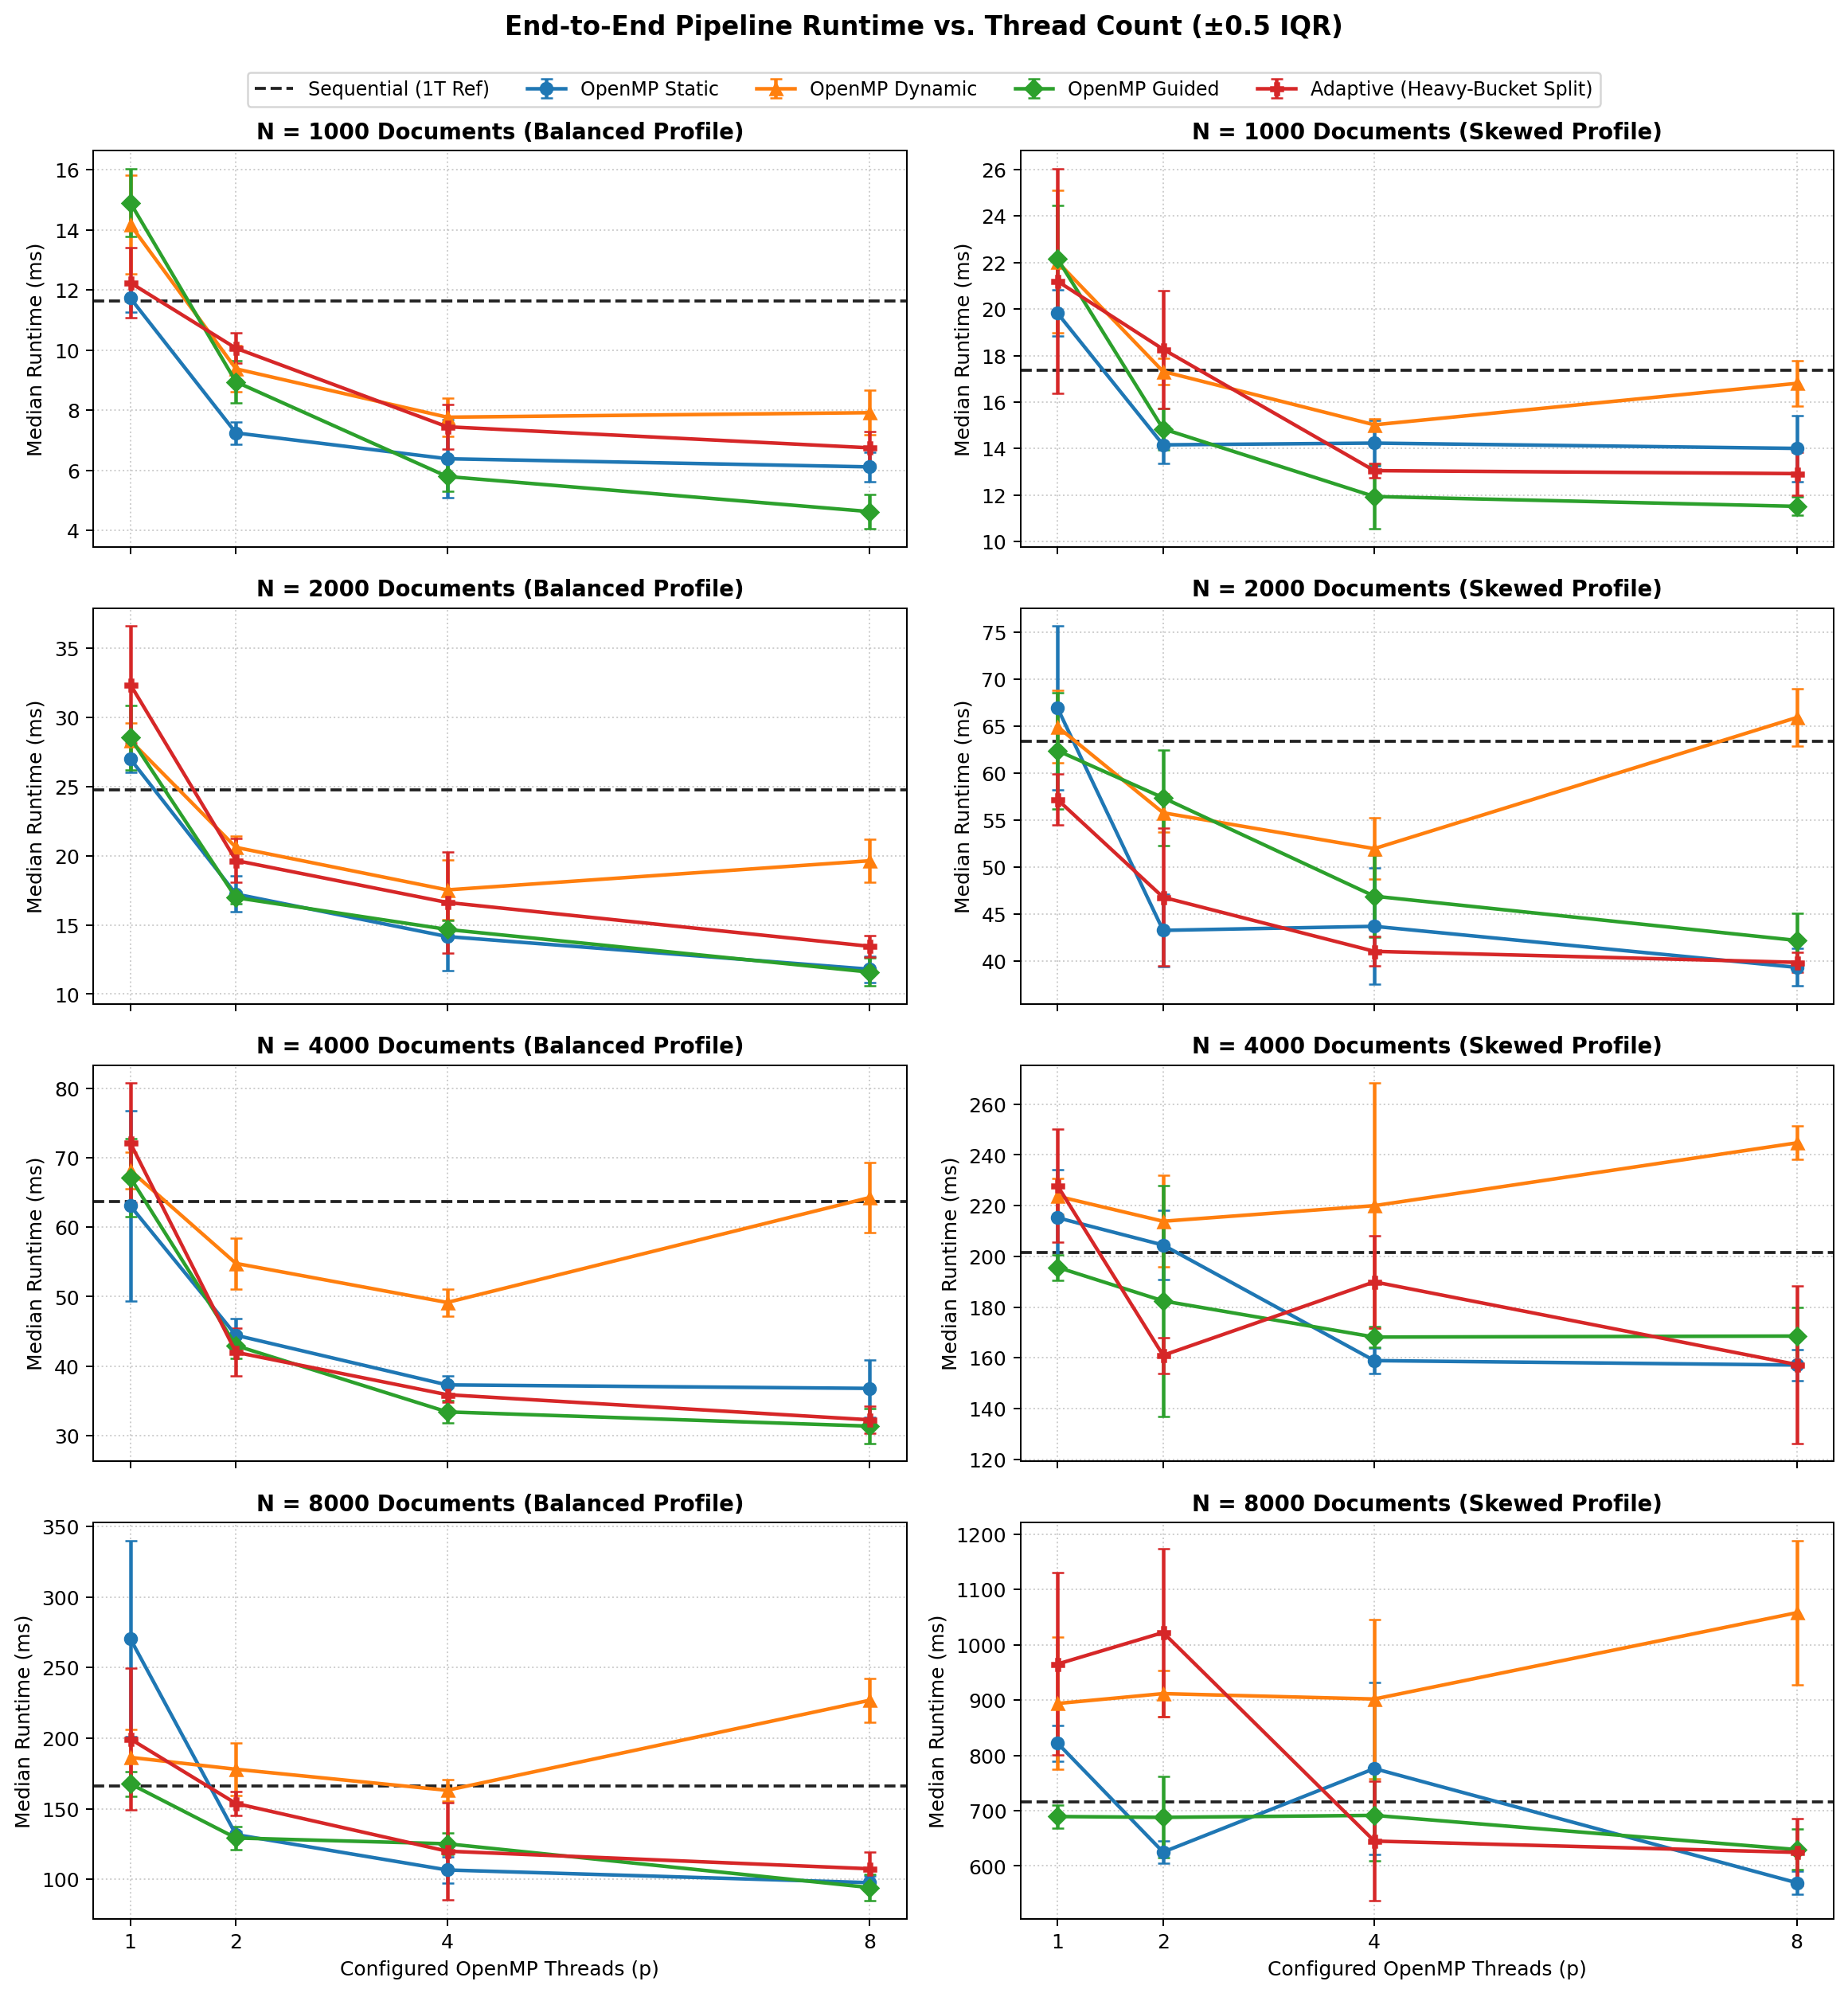
\includegraphics[height=0.37\textheight,keepaspectratio]{results/runtime_vs_threads.png}
    \caption*{Figure 1: Initial Baseline End-to-End Runtime vs Thread Count (Pre-Aggregation Parallelization)}
\end{figure}

\begin{figure}[H]
    \centering
    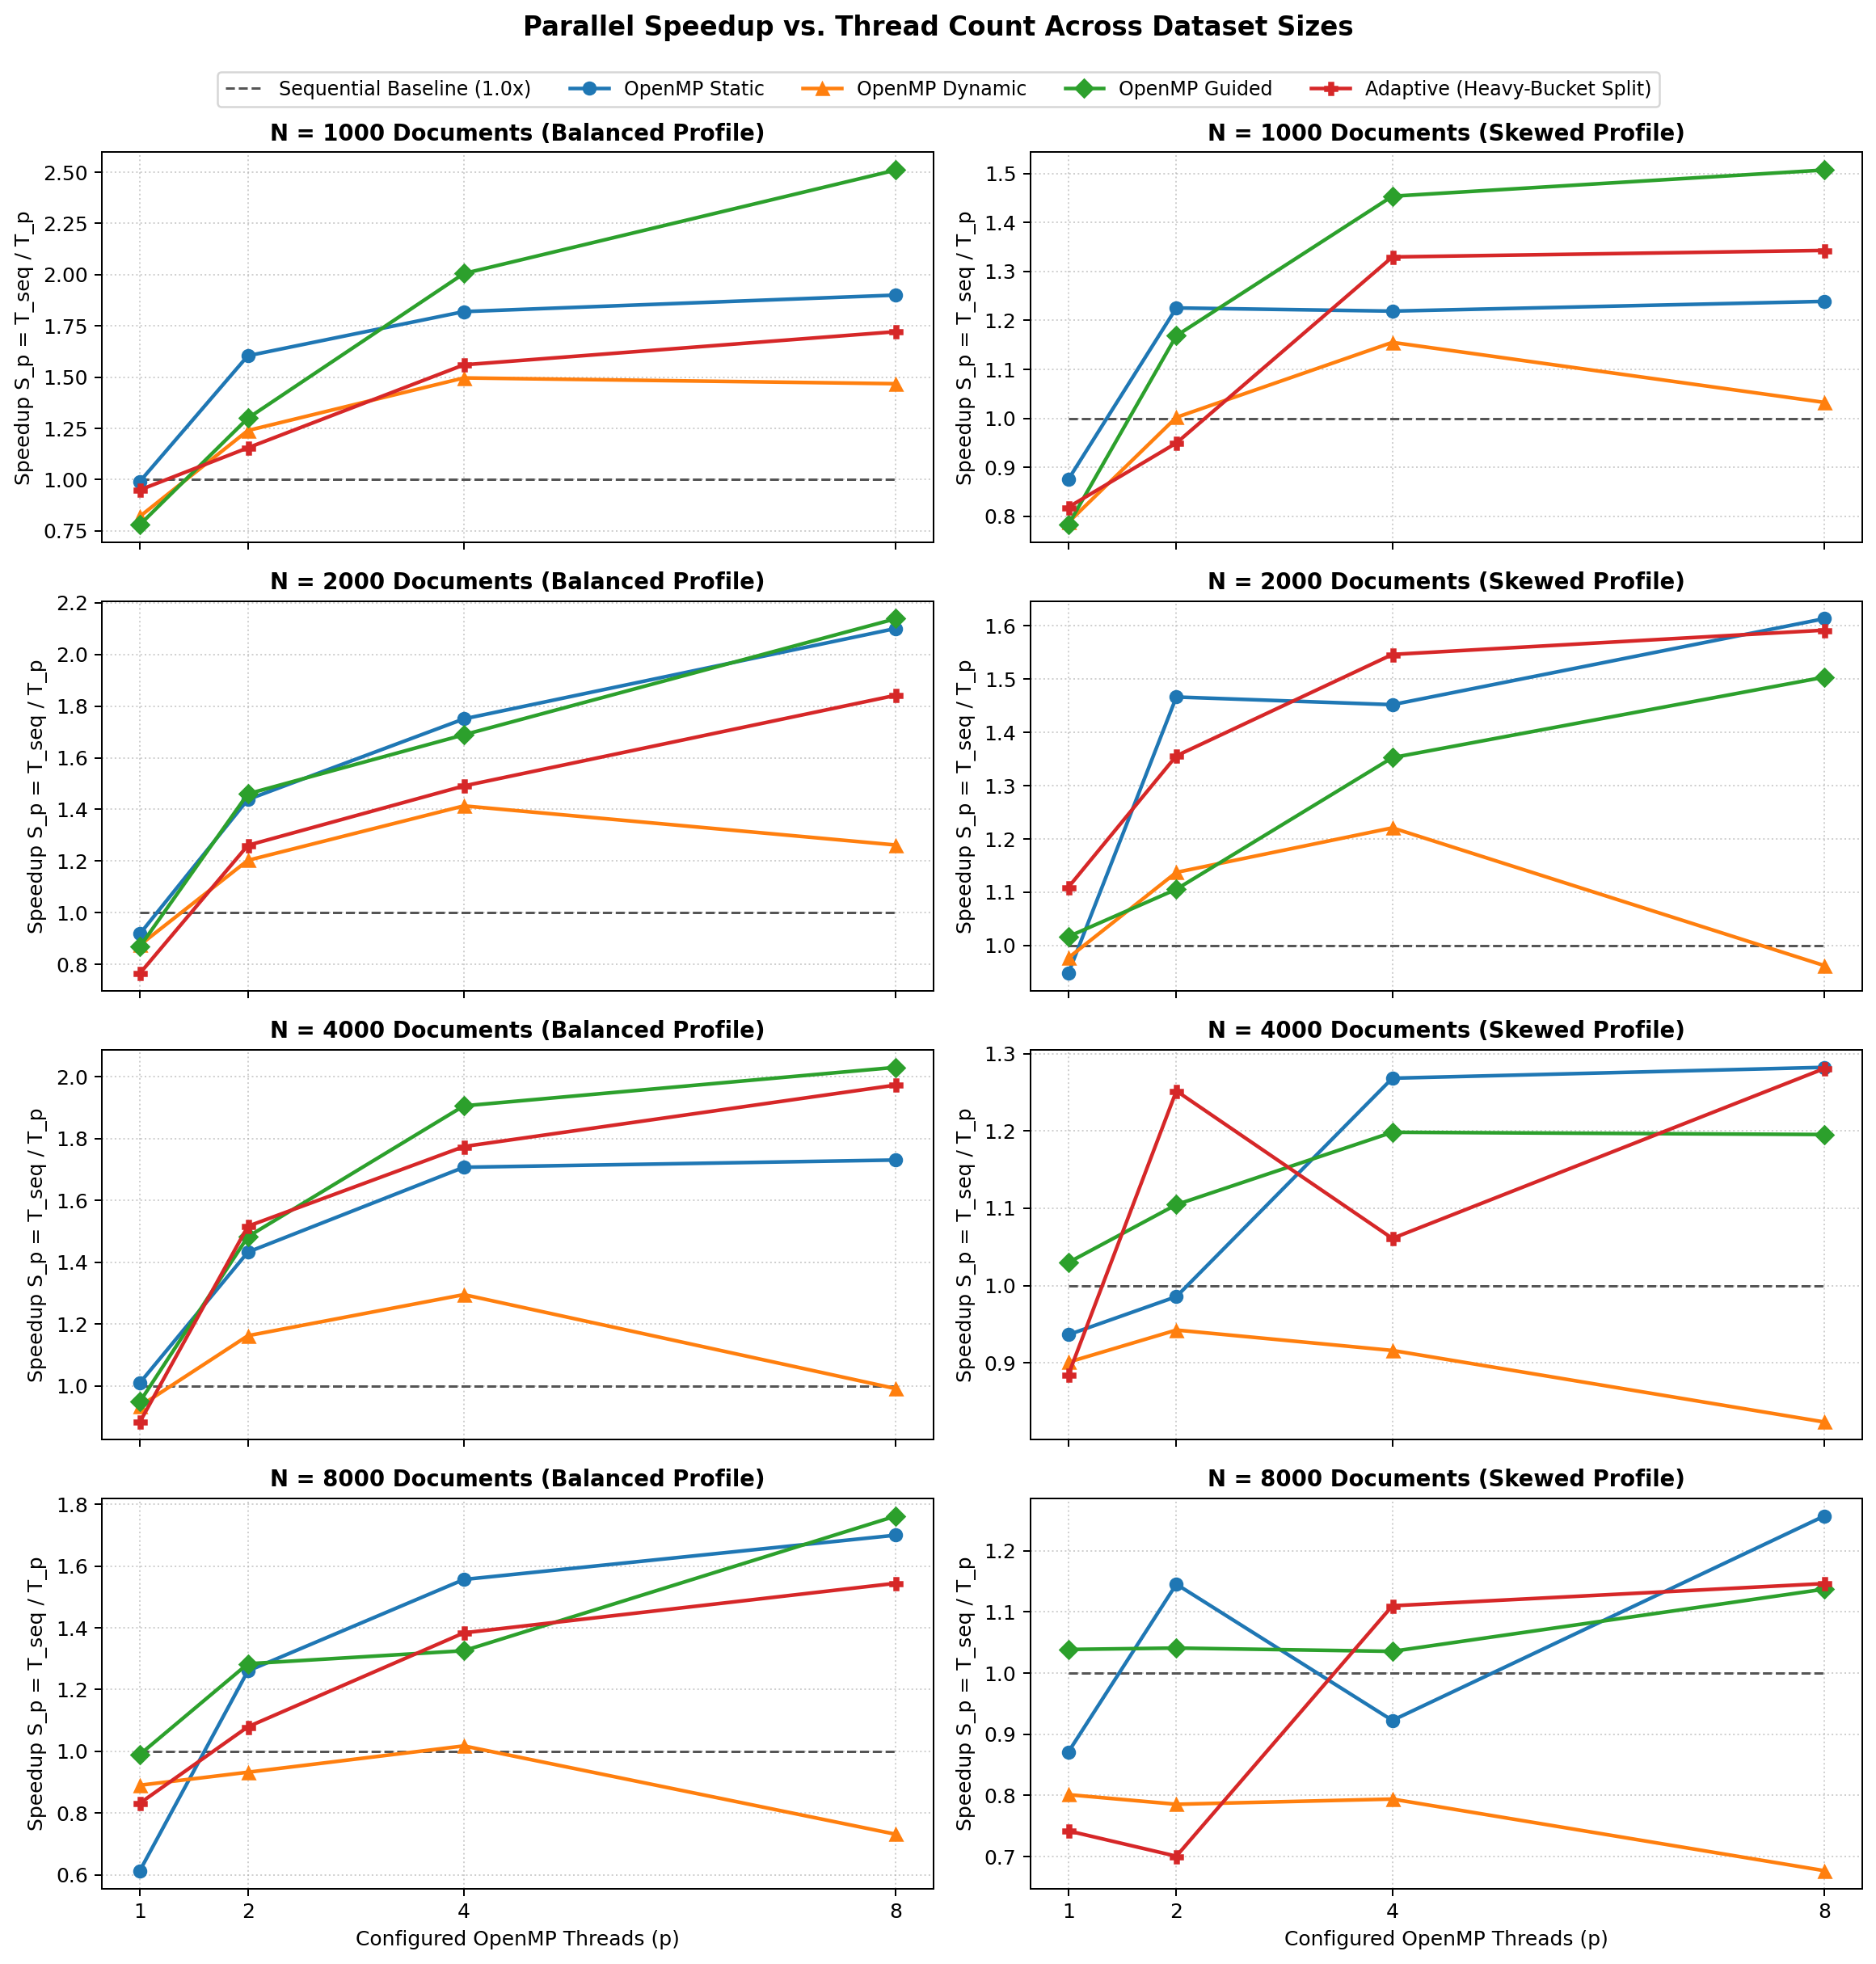
\includegraphics[height=0.43\textheight,keepaspectratio]{results/speedup_vs_threads.png}
    \caption*{Figure 2: Initial Baseline Parallel Speedup vs Thread Count (Pre-Aggregation Parallelization)}
\end{figure}

\begin{figure}[H]
    \centering
    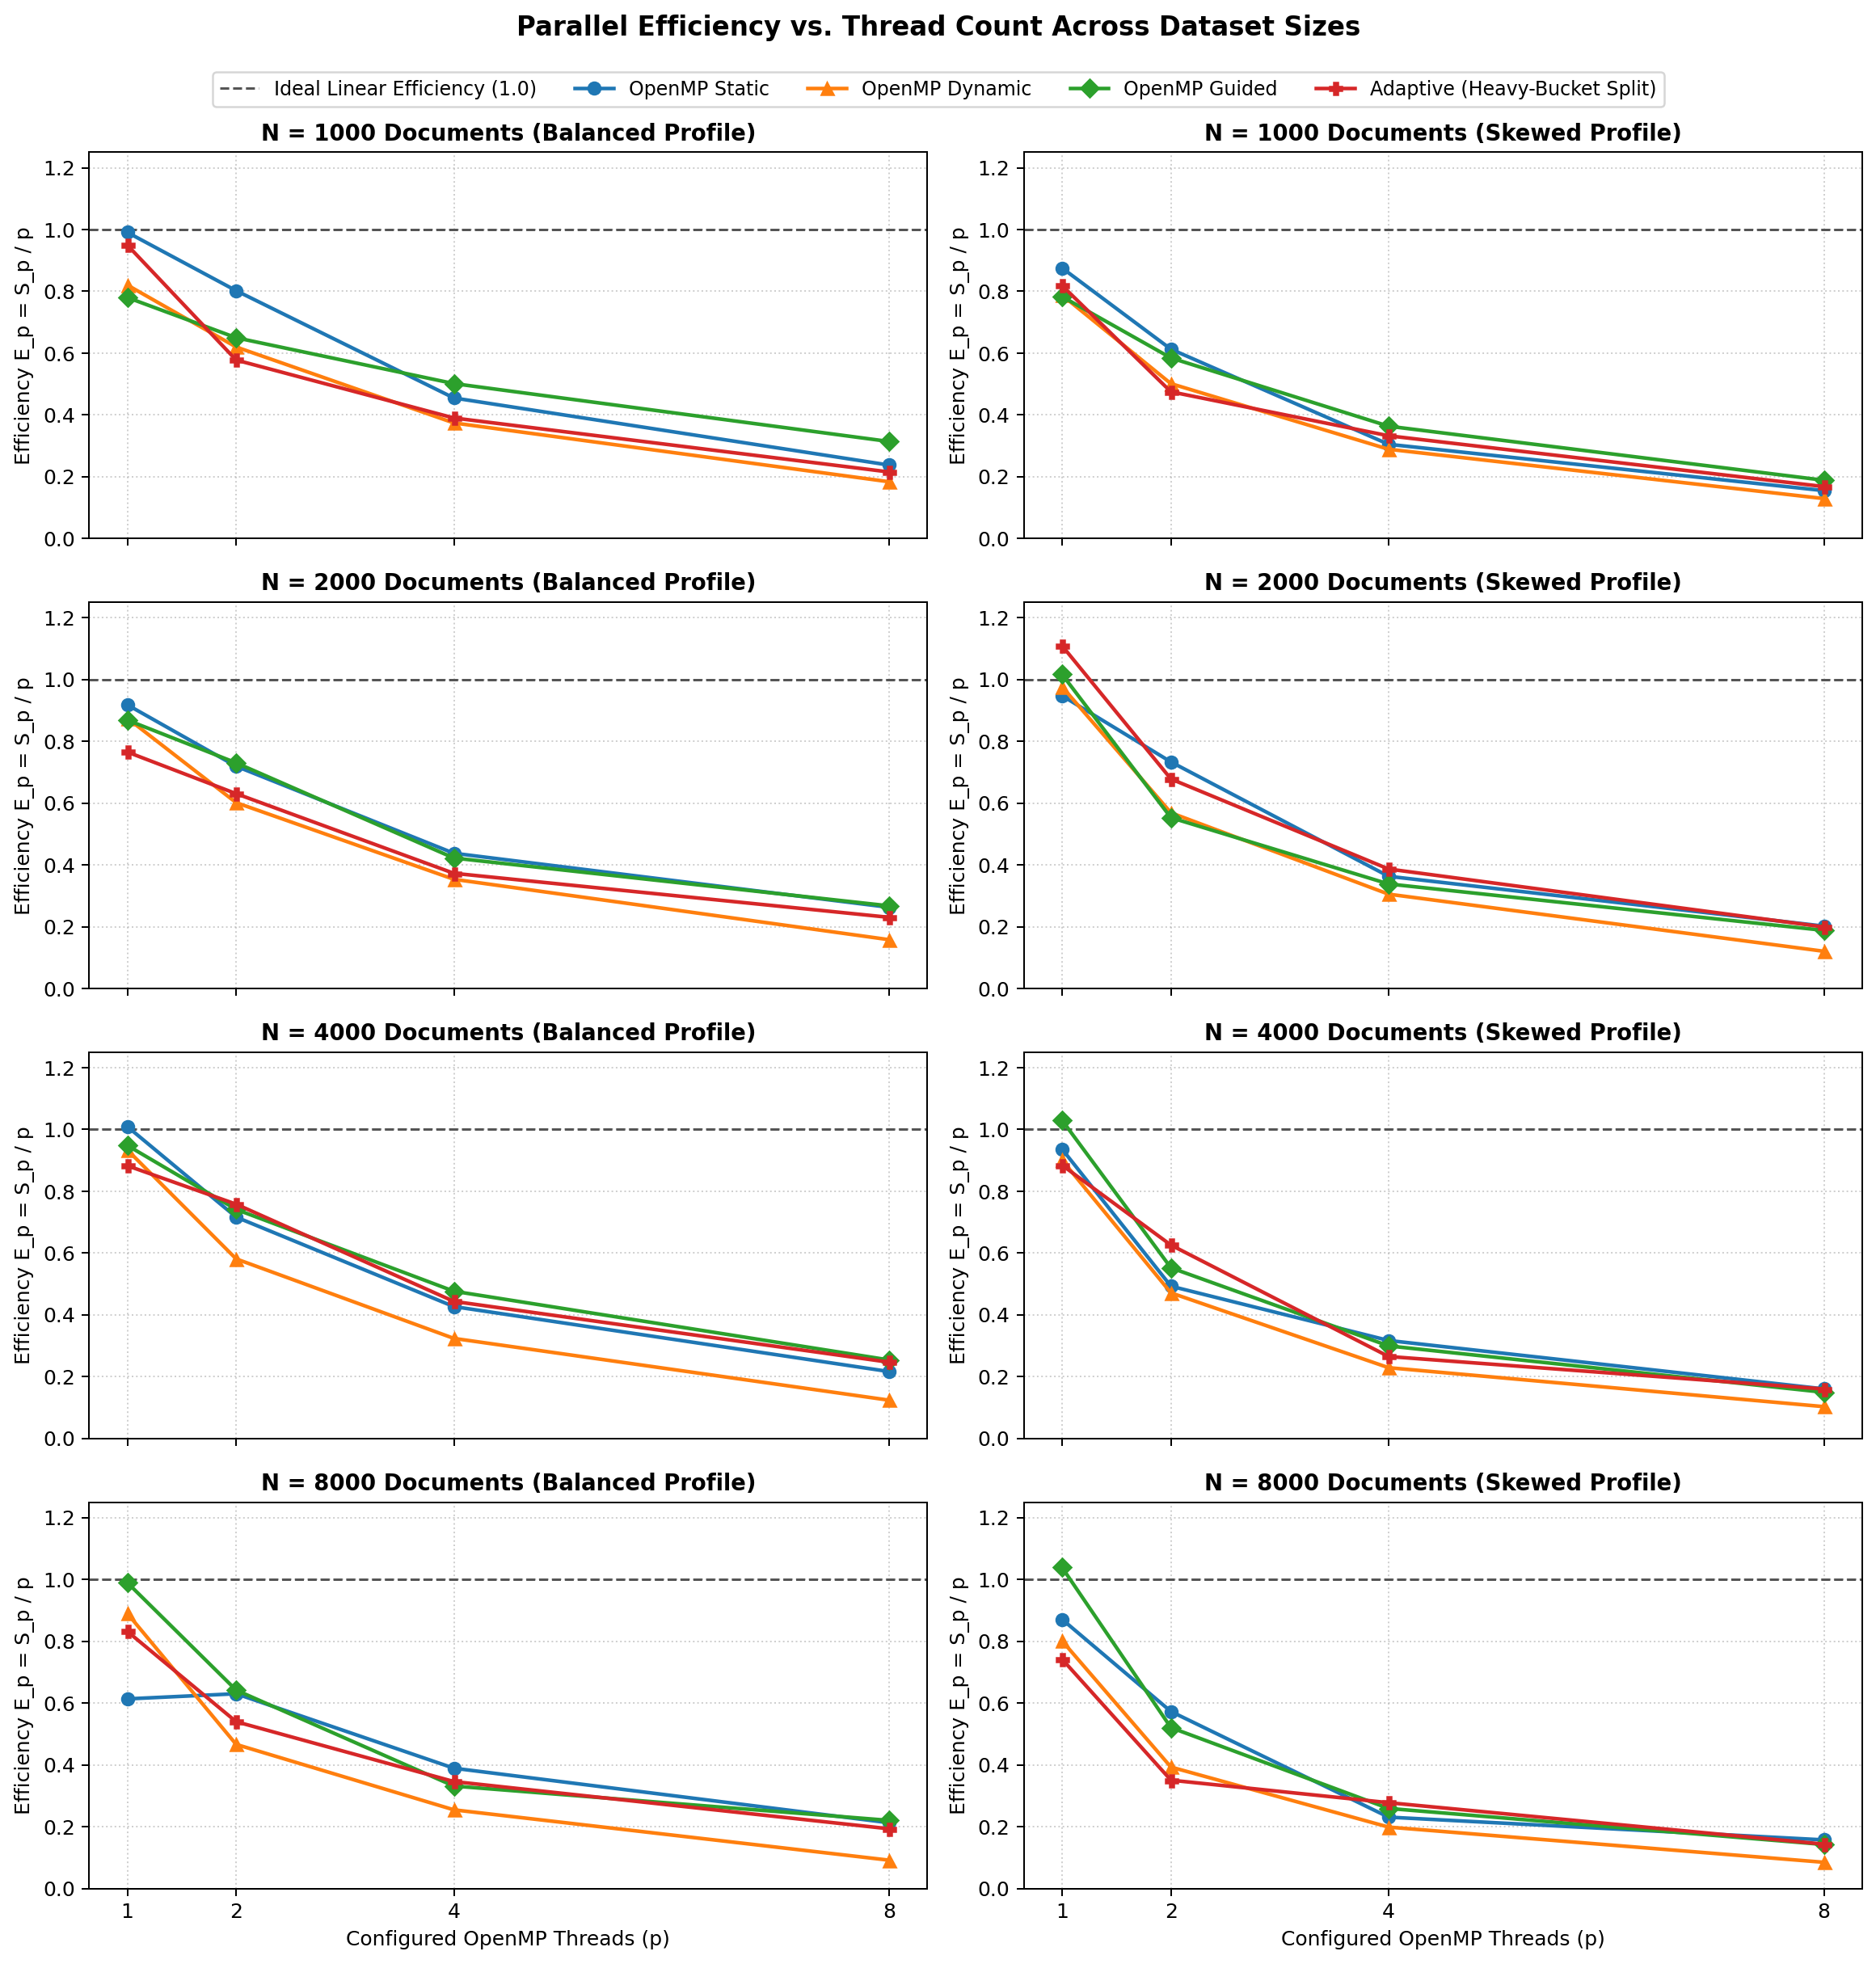
\includegraphics[height=0.43\textheight,keepaspectratio]{results/efficiency_vs_threads.png}
    \caption*{Figure 3: Initial Baseline Parallel Efficiency vs Thread Count (Pre-Aggregation Parallelization)}
\end{figure}

\begin{figure}[H]
    \centering
    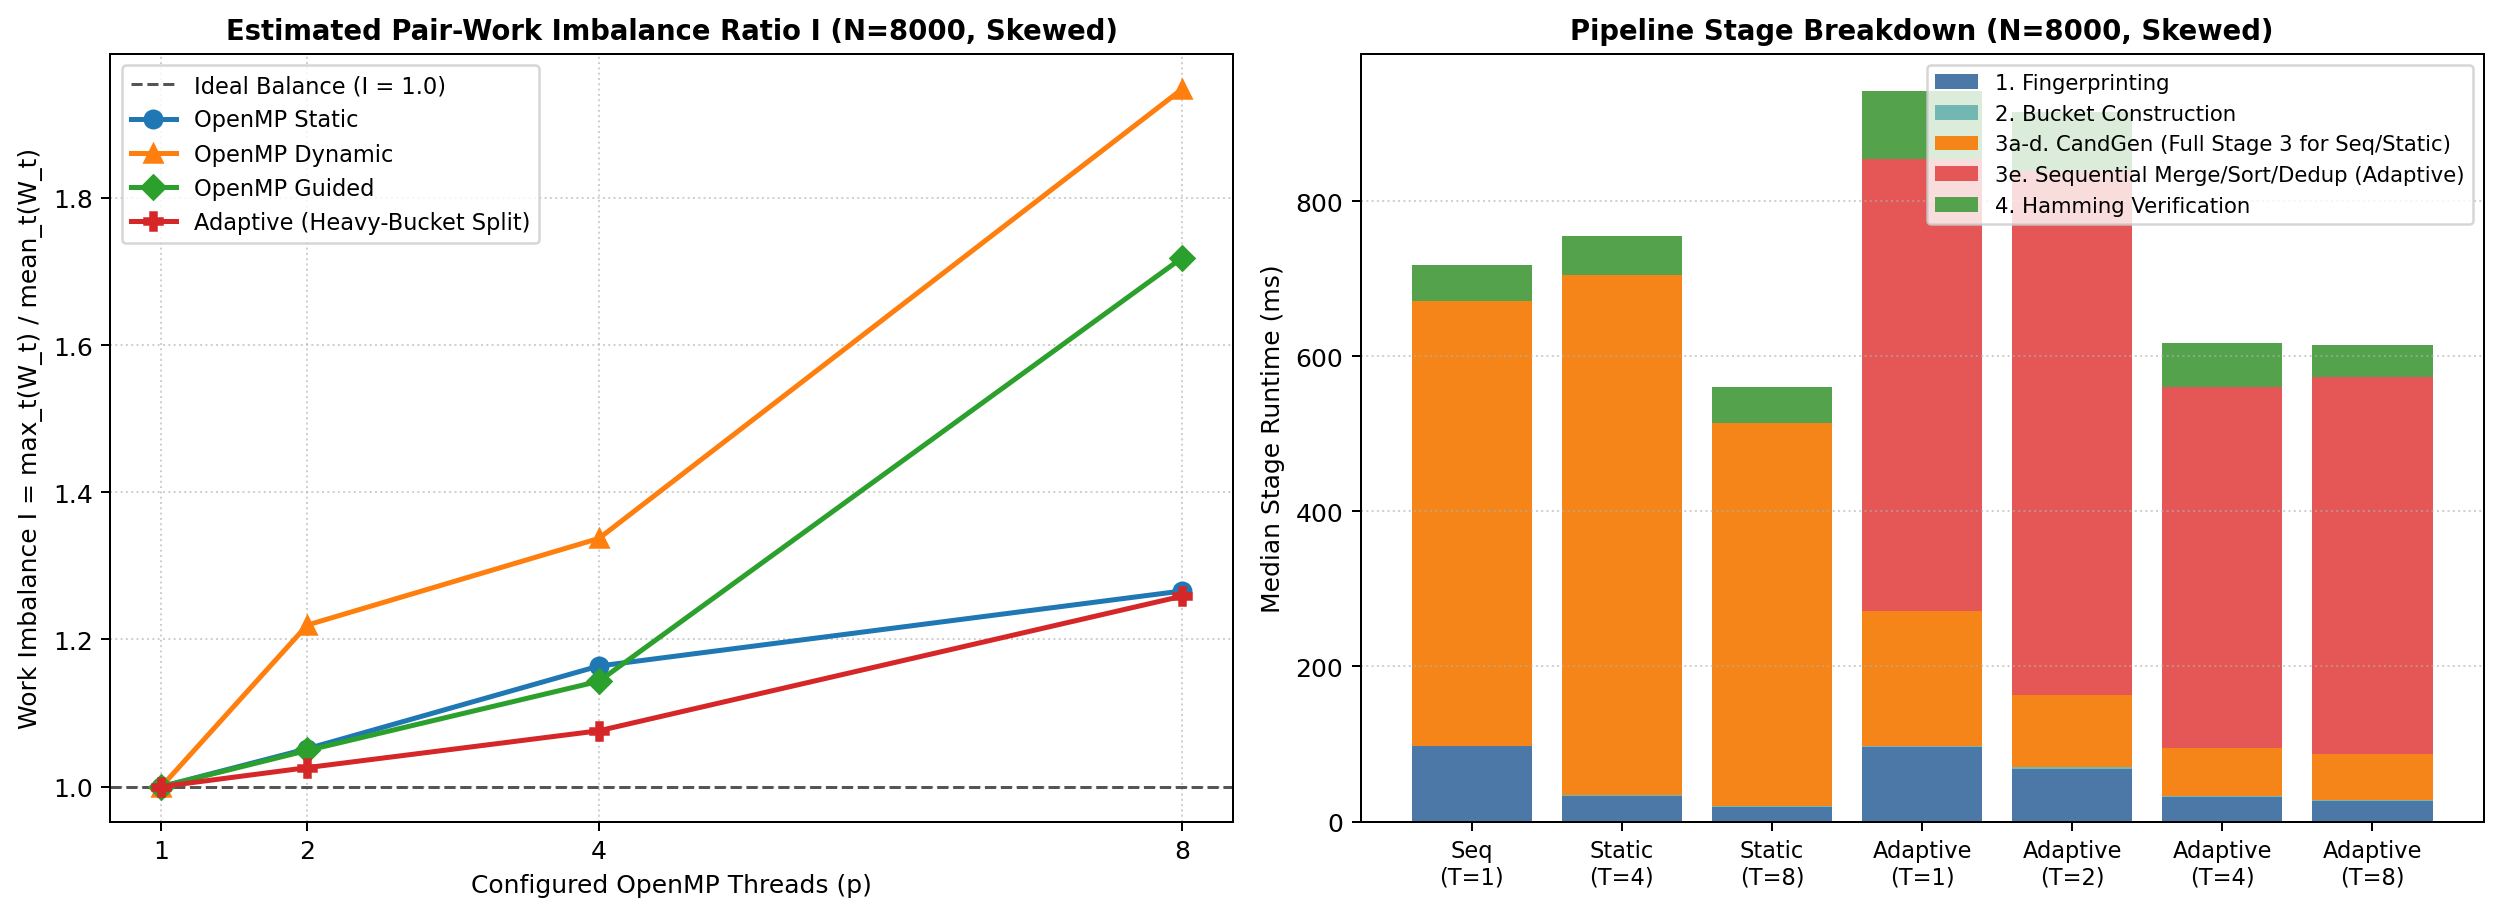
\includegraphics[width=0.92\textwidth]{results/work_imbalance_and_stages.png}
    \caption*{Figure 4: Estimated Pair-Work Imbalance Ratio and Stage Breakdown at N=8000 Skewed (Pre-Aggregation Parallelization)}
\end{figure}

\textit{What Figures 1--4 show:} In the right panel of \textbf{Figure 4} (\texttt{N = 8,000 Skewed}), parallel fingerprinting (\texttt{Stage 1}, blue) and heavy-chunk processing (\texttt{Stage 3a--d}, orange) scaled down cleanly from $1$ to $8$ threads, but sequential \texttt{Stage 3e} (\texttt{Merge, Sort \& Dedup}, red) took $465\text{--}668\text{ ms}$ regardless of thread count, acting as a serial bottleneck. \textbf{Table 2} compares the Phase 8 full benchmark (\texttt{results/phase8\_full\_summary.csv}) directly against Phase 9 (\texttt{results/phase9\_agg\_summary.csv}), where Stage 3e was parallelized using \texttt{aggregate\_and\_deduplicate\_candidates()}.

\begin{table}[H]
\centering
\caption*{Table 2: Effect of Parallel Range-Partitioned Candidate Merging and Deduplication at $N = 8,000$ (Phase 8 Serial Stage 3e vs.\ Phase 9 Parallel Stage 3e)}
\setlength{\tabcolsep}{4pt}
\renewcommand{\arraystretch}{1.15}
\resizebox{\textwidth}{!}{%
\rowcolors{2}{rowalt}{white}
\begin{tabular}{l l r r r r r r r r r c}
\toprule
\rowcolor{headbg}
\thead{Profile} & \thead{Policy} & \thead{Threads\\($T$)} & \thead{Phase 8\\Total (ms)} & \thead{Phase 9\\Total (ms)} & \thead{Total\\Change (\%)} & \thead{Phase 8\\Stage 3 (ms)} & \thead{Phase 9\\Stage 3 (ms)} & \thead{Phase 8\\Stage 3e (ms)} & \thead{Phase 9\\Stage 3e (ms)} & \thead{Stage 3e\\Change (\%)} & \thead{Speedup\\(P8 $\to$ P9)} \\
\midrule
\textbf{Skewed} & \texttt{Sequential} & 1 & 639.993 & 615.692 & -3.8\% & 525.757 & 491.535 & --- & --- & --- & 1.00x $\to$ 1.00x \\
\textbf{Skewed} & \texttt{Static} & 4 & 649.624 & 347.083 & \textbf{-46.6\%} & 563.453 & 269.723 & --- & --- & --- & 0.99x $\to$ \textbf{1.77x} \\
\textbf{Skewed} & \texttt{Static} & 8 & 546.594 & 293.164 & \textbf{-46.4\%} & 472.271 & 224.769 & --- & --- & --- & 1.17x $\to$ \textbf{2.10x} \\
\textbf{Skewed} & \texttt{Guided} & 4 & 672.727 & 424.540 & \textbf{-36.9\%} & 522.476 & 282.351 & --- & --- & --- & 0.95x $\to$ \textbf{1.45x} \\
\textbf{Skewed} & \texttt{Guided} & 8 & 636.014 & 363.936 & \textbf{-42.8\%} & 531.456 & 241.428 & --- & --- & --- & 1.01x $\to$ \textbf{1.69x} \\
\textbf{Skewed} & \texttt{Adaptive} & 1 & 755.265 & 649.626 & \textbf{-14.0\%} & 589.480 & 501.324 & 479.202 & 390.007 & \textbf{-18.6\%} & 0.85x $\to$ 0.95x \\
\textbf{Skewed} & \texttt{Adaptive} & 2 & 656.319 & 512.824 & \textbf{-21.9\%} & 558.632 & 405.415 & 475.044 & 324.633 & \textbf{-31.7\%} & 0.98x $\to$ \textbf{1.20x} \\
\textbf{Skewed} & \texttt{Adaptive} & 4 & 629.816 & 377.280 & \textbf{-40.1\%} & 544.617 & 288.912 & 481.103 & 222.740 & \textbf{-53.7\%} & 1.02x $\to$ \textbf{1.63x} \\
\textbf{Skewed} & \texttt{Adaptive} & 8 & 587.444 & 295.329 & \textbf{-49.7\%} & 519.874 & 227.087 & 465.336 & 171.106 & \textbf{-63.2\%} & 1.09x $\to$ \textbf{2.08x} \\
\textbf{Balanced} & \texttt{Sequential} & 1 & 166.274 & 185.322 & +11.5\% & 70.340 & 76.178 & --- & --- & --- & 1.00x $\to$ 1.00x \\
\textbf{Balanced} & \texttt{Static} & 8 & 100.030 & 57.683 & \textbf{-42.3\%} & 64.761 & 31.131 & --- & --- & --- & 1.66x $\to$ \textbf{3.21x} \\
\textbf{Balanced} & \texttt{Guided} & 8 & 100.946 & 60.175 & \textbf{-40.4\%} & 64.231 & 33.964 & --- & --- & --- & 1.65x $\to$ \textbf{3.08x} \\
\textbf{Balanced} & \texttt{Adaptive} & 4 & 106.601 & 82.846 & \textbf{-22.3\%} & 70.385 & 39.620 & 62.542 & 30.948 & \textbf{-50.5\%} & 1.56x $\to$ \textbf{2.24x} \\
\textbf{Balanced} & \texttt{Adaptive} & 8 & 101.049 & 61.666 & \textbf{-39.0\%} & 66.546 & 33.019 & 58.338 & 24.738 & \textbf{-57.6\%} & 1.65x $\to$ \textbf{3.01x} \\
\bottomrule
\end{tabular}%
}
\end{table}

\textit{What Table 2 shows:} Parallelizing Stage 3e cut \texttt{Adaptive} merge/dedup time on $N=8,000$ \texttt{Skewed} ($T=8$) from $465.336\text{ ms}$ down to $171.106\text{ ms}$ ($-63.2\%$, a $2.72\times$ stage speedup). This reduced total \texttt{Adaptive} runtime by almost half ($587.444\text{ ms} \to 295.329\text{ ms}$, $-49.7\%$) and nearly doubled total speedup from $1.09\times$ to $2.08\times$. Even at $T=1$, \texttt{Adaptive} Stage 3e got $18.6\%$ faster ($479.202\text{ ms} \to 390.007\text{ ms}$) because the single-thread fast path moves the buffer directly (\texttt{std::move}) instead of allocating and copying a second $137.85\text{ MB}$ vector. On $N=8,000$ \texttt{Balanced} ($T=8$), \texttt{Adaptive} Stage 3e time dropped by $57.6\%$ ($58.338\text{ ms} \to 24.738\text{ ms}$), increasing total speedup from $1.65\times$ to $3.01\times$.

\subsubsection*{3. Comparing Scheduling Policies and Load Balance}
\textbf{Table 3} compares baseline (\texttt{enable\_band\_suppression = false}) performance across all five policies (\texttt{Sequential}, \texttt{Static}, \texttt{Dynamic}, \texttt{Guided}, and \texttt{Adaptive}) at $N \in \{2000, 4000, 8000\}$ for $T \in \{4, 8\}$ (and $T=1$ for \texttt{Sequential}) from \texttt{results/phase10\_full\_paired\_summary.csv}.

\begin{table}[H]
\centering
\caption*{Table 3: Cross-Policy Baseline Performance, Speedup, Efficiency, and Work Imbalance ($N = 2,000, 4,000, 8,000$, Baseline Mode \texttt{Supp=0})}
\setlength{\tabcolsep}{5.2pt}
\renewcommand{\arraystretch}{0.95}
\renewcommand\cellgape{\Gape[0pt]}
\resizebox{\textwidth}{!}{%
\rowcolors{2}{rowalt}{white}
\begin{tabular}{r l l c r r r r r r c c}
\toprule
\rowcolor{headbg}
\thead{$N$} & \thead{Profile} & \thead{Policy} & \thead{Threads\\($T$)} & \thead{Median\\Total (ms)} & \thead{IQR\\Total (ms)} & \thead{Median\\Stage 3 (ms)} & \thead{Speedup\\($S_p$)} & \thead{Efficiency\\($E_p$)} & \thead{Work\\Imbalance ($I$)} & \thead{Part.\\Threads} & \thead{Parity} \\
\midrule
\textbf{2000} & Balanced & \texttt{Sequential} & 1 & 26.664 & 3.410 & 4.757 & 1.00x & 1.00 & 1.000 & 1/1 & PASS \\
\textbf{2000} & Balanced & \texttt{Static} & 4 / 8 & \makecell[r]{13.225 /\\ 12.989} & \makecell[r]{4.617 /\\ 2.137} & \makecell[r]{3.611 /\\ 3.238} & \makecell[r]{2.02x /\\ 2.05x} & \makecell[r]{0.50 /\\ 0.26} & \makecell[r]{1.024 /\\ 1.047} & \makecell[c]{4/4,\\ 8/8} & PASS \\
\textbf{2000} & Balanced & \texttt{Dynamic} & 4 / 8 & \makecell[r]{16.771 /\\ 21.164} & \makecell[r]{0.640 /\\ 2.762} & \makecell[r]{3.562 /\\ 2.971} & \makecell[r]{1.59x /\\ 1.26x} & \makecell[r]{0.40 /\\ 0.16} & \makecell[r]{1.192 /\\ 1.354} & \makecell[c]{4/4,\\ 8/8} & PASS \\
\textbf{2000} & Balanced & \texttt{Guided} & 4 / 8 & \makecell[r]{13.891 /\\ 12.015} & \makecell[r]{4.076 /\\ 1.510} & \makecell[r]{3.230 /\\ 2.974} & \makecell[r]{1.92x /\\ 2.22x} & \makecell[r]{0.48 /\\ 0.28} & \makecell[r]{1.405 /\\ 1.933} & \makecell[c]{4/4,\\ \textbf{6/8}} & PASS \\
\textbf{2000} & Balanced & \texttt{Adaptive} & 4 / 8 & \makecell[r]{14.131 /\\ \textbf{11.946}} & \makecell[r]{4.680 /\\ 4.956} & \makecell[r]{3.461 /\\ \textbf{2.949}} & \makecell[r]{1.89x /\\ \textbf{2.23x}} & \makecell[r]{0.47 /\\ \textbf{0.28}} & \makecell[r]{1.124 /\\ 1.318} & \makecell[c]{4/4,\\ 8/8} & PASS \\
\textbf{2000} & Skewed & \texttt{Sequential} & 1 & 63.524 & 20.277 & 36.925 & 1.00x & 1.00 & 1.000 & 1/1 & PASS \\
\textbf{2000} & Skewed & \texttt{Static} & 4 / 8 & \makecell[r]{30.665 /\\ \textbf{26.411}} & \makecell[r]{9.160 /\\ 10.377} & \makecell[r]{18.396 /\\ \textbf{15.017}} & \makecell[r]{2.07x /\\ \textbf{2.41x}} & \makecell[r]{0.52 /\\ \textbf{0.30}} & \makecell[r]{1.171 /\\ 1.315} & \makecell[c]{4/4,\\ 8/8} & PASS \\
\textbf{2000} & Skewed & \texttt{Dynamic} & 4 / 8 & \makecell[r]{38.885 /\\ 51.597} & \makecell[r]{32.574 /\\ 6.344} & \makecell[r]{18.391 /\\ 16.545} & \makecell[r]{1.63x /\\ 1.23x} & \makecell[r]{0.41 /\\ 0.15} & \makecell[r]{1.318 /\\ 1.685} & \makecell[c]{4/4,\\ \textbf{7/8}} & PASS \\
\textbf{2000} & Skewed & \texttt{Guided} & 4 / 8 & \makecell[r]{32.522 /\\ 26.817} & \makecell[r]{16.369 /\\ 8.950} & \makecell[r]{19.632 /\\ 15.647} & \makecell[r]{1.95x /\\ 2.37x} & \makecell[r]{0.49 /\\ 0.30} & \makecell[r]{1.404 /\\ 1.694} & \makecell[c]{4/4,\\ 8/8} & PASS \\
\textbf{2000} & Skewed & \texttt{Adaptive} & 4 / 8 & \makecell[r]{\textbf{29.486} /\\ 28.021} & \makecell[r]{5.269 /\\ 5.271} & \makecell[r]{\textbf{18.272} /\\ 16.844} & \makecell[r]{\textbf{2.15x} /\\ 2.27x} & \makecell[r]{\textbf{0.54} /\\ 0.28} & \makecell[r]{\textbf{1.067} /\\ \textbf{1.275}} & \makecell[c]{4/4,\\ 8/8} & PASS \\
\textbf{4000} & Balanced & \texttt{Sequential} & 1 & 63.955 & 10.229 & 20.301 & 1.00x & 1.00 & 1.000 & 1/1 & PASS \\
\textbf{4000} & Balanced & \texttt{Static} & 4 / 8 & \makecell[r]{27.415 /\\ 22.799} & \makecell[r]{5.134 /\\ 3.829} & \makecell[r]{9.687 /\\ 8.368} & \makecell[r]{2.33x /\\ 2.81x} & \makecell[r]{0.58 /\\ 0.35} & \makecell[r]{1.008 /\\ 1.010} & \makecell[c]{4/4,\\ 8/8} & PASS \\
\textbf{4000} & Balanced & \texttt{Dynamic} & 4 / 8 & \makecell[r]{39.858 /\\ 55.456} & \makecell[r]{5.577 /\\ 8.766} & \makecell[r]{9.301 /\\ 7.775} & \makecell[r]{1.60x /\\ 1.15x} & \makecell[r]{0.40 /\\ 0.14} & \makecell[r]{1.118 /\\ 1.450} & \makecell[c]{4/4,\\ 8/8} & PASS \\
\textbf{4000} & Balanced & \texttt{Guided} & 4 / 8 & \makecell[r]{\textbf{25.523} /\\ \textbf{21.148}} & \makecell[r]{3.538 /\\ 0.544} & \makecell[r]{9.663 /\\ 8.935} & \makecell[r]{\textbf{2.51x} /\\ \textbf{3.02x}} & \makecell[r]{\textbf{0.63} /\\ \textbf{0.38}} & \makecell[r]{1.069 /\\ 1.446} & \makecell[c]{4/4,\\ 8/8} & PASS \\
\textbf{4000} & Balanced & \texttt{Adaptive} & 4 / 8 & \makecell[r]{28.755 /\\ 30.937} & \makecell[r]{3.572 /\\ 10.360} & \makecell[r]{10.170 /\\ 10.025} & \makecell[r]{2.22x /\\ 2.07x} & \makecell[r]{0.56 /\\ 0.26} & \makecell[r]{1.017 /\\ 1.067} & \makecell[c]{4/4,\\ 8/8} & PASS \\
\textbf{4000} & Skewed & \texttt{Sequential} & 1 & 177.805 & 27.381 & 125.325 & 1.00x & 1.00 & 1.000 & 1/1 & PASS \\
\textbf{4000} & Skewed & \texttt{Static} & 4 / 8 & \makecell[r]{99.205 /\\ \textbf{77.101}} & \makecell[r]{3.521 /\\ 9.041} & \makecell[r]{70.295 /\\ 57.183} & \makecell[r]{1.79x /\\ \textbf{2.31x}} & \makecell[r]{0.45 /\\ \textbf{0.29}} & \makecell[r]{1.172 /\\ 1.261} & \makecell[c]{4/4,\\ 8/8} & PASS \\
\textbf{4000} & Skewed & \texttt{Dynamic} & 4 / 8 & \makecell[r]{139.115 /\\ 166.899} & \makecell[r]{8.891 /\\ 16.445} & \makecell[r]{70.090 /\\ 53.278} & \makecell[r]{1.28x /\\ 1.07x} & \makecell[r]{0.32 /\\ 0.13} & \makecell[r]{1.232 /\\ 1.643} & \makecell[c]{4/4,\\ 8/8} & PASS \\
\textbf{4000} & Skewed & \texttt{Guided} & 4 / 8 & \makecell[r]{98.266 /\\ 85.608} & \makecell[r]{18.931 /\\ 1.623} & \makecell[r]{68.363 /\\ 56.046} & \makecell[r]{1.81x /\\ 2.08x} & \makecell[r]{0.45 /\\ 0.26} & \makecell[r]{1.545 /\\ 1.739} & \makecell[c]{4/4,\\ 8/8} & PASS \\
\textbf{4000} & Skewed & \texttt{Adaptive} & 4 / 8 & \makecell[r]{\textbf{97.974} /\\ 82.857} & \makecell[r]{6.446 /\\ 4.266} & \makecell[r]{69.064 /\\ 57.482} & \makecell[r]{\textbf{1.81x} /\\ 2.15x} & \makecell[r]{\textbf{0.45} /\\ 0.27} & \makecell[r]{\textbf{1.181} /\\ 1.281} & \makecell[c]{4/4,\\ 8/8} & PASS \\
\textbf{8000} & Balanced & \texttt{Sequential} & 1 & 162.182 & 17.928 & 69.746 & 1.00x & 1.00 & 1.000 & 1/1 & PASS \\
\textbf{8000} & Balanced & \texttt{Static} & 4 / 8 & \makecell[r]{83.379 /\\ 63.538} & \makecell[r]{14.920 /\\ 12.775} & \makecell[r]{38.304 /\\ 31.117} & \makecell[r]{1.95x /\\ 2.55x} & \makecell[r]{0.49 /\\ 0.32} & \makecell[r]{1.009 /\\ 1.011} & \makecell[c]{4/4,\\ 8/8} & PASS \\
\textbf{8000} & Balanced & \texttt{Dynamic} & 4 / 8 & \makecell[r]{132.386 /\\ 219.875} & \makecell[r]{18.519 /\\ 62.434} & \makecell[r]{36.016 /\\ 31.269} & \makecell[r]{1.23x /\\ 0.74x} & \makecell[r]{0.31 /\\ 0.09} & \makecell[r]{1.089 /\\ 1.433} & \makecell[c]{4/4,\\ 8/8} & PASS \\
\textbf{8000} & Balanced & \texttt{Guided} & 4 / 8 & \makecell[r]{\textbf{74.782} /\\ \textbf{52.741}} & \makecell[r]{7.326 /\\ 6.621} & \makecell[r]{37.105 /\\ 30.193} & \makecell[r]{\textbf{2.17x} /\\ \textbf{3.08x}} & \makecell[r]{\textbf{0.54} /\\ \textbf{0.38}} & \makecell[r]{1.149 /\\ 1.199} & \makecell[c]{4/4,\\ 8/8} & PASS \\
\textbf{8000} & Balanced & \texttt{Adaptive} & 4 / 8 & \makecell[r]{81.811 /\\ 60.893} & \makecell[r]{6.206 /\\ 6.515} & \makecell[r]{38.729 /\\ \textbf{30.075}} & \makecell[r]{1.98x /\\ 2.66x} & \makecell[r]{0.50 /\\ 0.33} & \makecell[r]{\textbf{1.007} /\\ \textbf{1.011}} & \makecell[c]{4/4,\\ 8/8} & PASS \\
\textbf{8000} & Skewed & \texttt{Sequential} & 1 & 656.054 & 153.099 & 511.836 & 1.00x & 1.00 & 1.000 & 1/1 & PASS \\
\textbf{8000} & Skewed & \texttt{Static} & 4 / 8 & \makecell[r]{376.132 /\\ \textbf{268.839}} & \makecell[r]{155.052 /\\ 174.559} & \makecell[r]{274.238 /\\ \textbf{202.216}} & \makecell[r]{1.74x /\\ \textbf{2.44x}} & \makecell[r]{0.44 /\\ \textbf{0.31}} & \makecell[r]{1.164 /\\ 1.266} & \makecell[c]{4/4,\\ 8/8} & PASS \\
\textbf{8000} & Skewed & \texttt{Dynamic} & 4 / 8 & \makecell[r]{616.609 /\\ 684.678} & \makecell[r]{437.803 /\\ 399.375} & \makecell[r]{289.416 /\\ 220.247} & \makecell[r]{1.06x /\\ 0.96x} & \makecell[r]{0.27 /\\ 0.12} & \makecell[r]{1.257 /\\ 1.590} & \makecell[c]{4/4,\\ 8/8} & PASS \\
\textbf{8000} & Skewed & \texttt{Guided} & 4 / 8 & \makecell[r]{\textbf{344.492} /\\ 313.773} & \makecell[r]{242.668 /\\ 29.107} & \makecell[r]{\textbf{262.624} /\\ 205.815} & \makecell[r]{\textbf{1.90x} /\\ 2.09x} & \makecell[r]{\textbf{0.48} /\\ 0.26} & \makecell[r]{1.131 /\\ 1.719} & \makecell[c]{4/4,\\ 8/8} & PASS \\
\textbf{8000} & Skewed & \texttt{Adaptive} & 4 / 8 & \makecell[r]{370.332 /\\ 294.950} & \makecell[r]{173.276 /\\ 41.199} & \makecell[r]{271.416 /\\ 218.987} & \makecell[r]{1.77x /\\ 2.22x} & \makecell[r]{0.44 /\\ 0.28} & \makecell[r]{\textbf{1.078} /\\ 1.308} & \makecell[c]{4/4,\\ 8/8} & PASS \\
\bottomrule
\end{tabular}%
}
\end{table}

\textit{What Table 3 shows:} On \texttt{Skewed} workloads at $T=4$ (which matches the 4 physical cores on the test CPU), \texttt{Adaptive} gets the lowest work imbalance ($I = 1.067$ at $N=2,000$ and $I = 1.078$ at $N=8,000$) and the fastest or tied-fastest median runtime at $N=2,000$ ($29.486\text{ ms}$, $2.15\times$) and $N=4,000$ ($97.974\text{ ms}$, $1.81\times$). At $T=8$, \texttt{Adaptive} ($294.950\text{ ms}$, $2.22\times$ at $N=8,000$) beats both \texttt{Guided} ($313.773\text{ ms}$, $2.09\times$, $I=1.719$) and \texttt{Dynamic} ($684.678\text{ ms}$, $0.96\times$, which is slower than single-threaded \texttt{Sequential} because of dynamic queue overhead in Stage 4), while staying within $9.7\%$ of \texttt{Static} ($268.839\text{ ms}$, $2.44\times$). Also, on $N=2,000$ \texttt{Balanced} ($T=8$) and $N=2,000$ \texttt{Skewed} ($T=8$), \texttt{Guided} and \texttt{Dynamic} leave 1--2 threads completely unused (\texttt{6/8} and \texttt{7/8} participating threads), while \texttt{Adaptive} uses all 8 threads (\texttt{8/8}) in every case.

\subsubsection*{4. Effect of Optional Band-Aware Candidate Suppression (Phase 10 Paired Benchmark)}
\textbf{Table 4} shows the paired in-process comparison (\texttt{-{}-compare-band-suppression}, \texttt{results/phase10\_full\_paired\_summary.csv}) between Baseline (\texttt{Supp=0}) and Band-Aware Candidate Suppression (\texttt{Supp=1}) across all five dataset sizes $N \in \{500, 1000, 2000, 4000, 8000\}$ for \texttt{Sequential} ($T=1$) and \texttt{Adaptive} ($T \in \{1, 2, 4, 8\}$), plus \texttt{Static}, \texttt{Dynamic}, and \texttt{Guided} at $N=8,000, T=8$.

\begin{table}[H]
\centering
\caption*{Table 4: Paired In-Process Comparison of Baseline (\texttt{Supp=0}) vs.\ Optional Band-Aware Candidate Suppression (\texttt{Supp=1}) Across $N = 500$ to $8,000$}
\setlength{\tabcolsep}{5.2pt}
\renewcommand{\arraystretch}{0.94}
\renewcommand\cellgape{\Gape[0.2pt]}
\resizebox{\textwidth}{!}{%
\rowcolors{2}{rowalt}{white}
\begin{tabular}{r l l c r r r r r r c}
\toprule
\rowcolor{headbg}
\thead{$N$} & \thead{Profile} & \thead{Policy} & \thead{Threads\\($T$)} & \thead{Baseline\\Total (ms)} & \thead{Suppression\\Total (ms)} & \thead{Total\\Change (\%)} & \thead{Baseline\\Stage 3 (ms)} & \thead{Suppression\\Stage 3 (ms)} & \thead{Stage 3e\\Base $\to$ Supp (ms)} & \thead{Speedup\\Base $\to$ Supp} \\
\midrule
\textbf{500} & Skewed & \texttt{Sequential} & 1 & 8.413 & 6.013 & \textbf{-28.5\%} & 1.776 & 0.621 (-65.0\%) & --- & 1.00x $\to$ 1.40x \\
\textbf{500} & Skewed & \texttt{Adaptive} & 1 / 2 & \makecell[r]{7.952 /\\ 7.067} & \makecell[r]{6.999 /\\ 6.120} & \makecell[r]{\textbf{-12.0\% /}\\ \textbf{-13.4\%}} & \makecell[r]{1.911 /\\ 1.673} & \makecell[r]{0.770 /\\ 1.004} & \makecell[r]{1.422 $\to$ 0.490 /\\ 1.247 $\to$ 0.587} & \makecell[c]{1.06x $\to$ 1.20x /\\ 1.19x $\to$ 1.37x} \\
\textbf{500} & Skewed & \texttt{Adaptive} & 4 / 8 & \makecell[r]{5.674 /\\ 6.078} & \makecell[r]{4.322 /\\ 4.104} & \makecell[r]{\textbf{-23.8\% /}\\ \textbf{-32.5\%}} & \makecell[r]{1.872 /\\ 1.958} & \makecell[r]{0.963 /\\ 1.403} & \makecell[r]{1.288 $\to$ 0.530 /\\ 1.029 $\to$ 0.642} & \makecell[c]{1.48x $\to$ 1.95x /\\ 1.38x $\to$ 2.05x} \\
\textbf{1000} & Skewed & \texttt{Sequential} & 1 & 17.612 & 13.150 & \textbf{-25.3\%} & 7.732 & 2.491 (-67.8\%) & --- & 1.00x $\to$ 1.34x \\
\textbf{1000} & Skewed & \texttt{Adaptive} & 1 / 2 & \makecell[r]{19.168 /\\ 13.882} & \makecell[r]{14.438 /\\ 10.990} & \makecell[r]{\textbf{-24.7\% /}\\ \textbf{-20.8\%}} & \makecell[r]{8.362 /\\ 6.328} & \makecell[r]{2.601 /\\ 2.423} & \makecell[r]{6.170 $\to$ 2.028 /\\ 4.770 $\to$ 1.817} & \makecell[c]{0.92x $\to$ 1.22x /\\ 1.27x $\to$ 1.60x} \\
\textbf{1000} & Skewed & \texttt{Adaptive} & 4 / 8 & \makecell[r]{12.795 /\\ 11.708} & \makecell[r]{8.541 /\\ 7.933} & \makecell[r]{\textbf{-33.3\% /}\\ \textbf{-32.2\%}} & \makecell[r]{5.910 /\\ 5.190} & \makecell[r]{1.931 /\\ 2.016} & \makecell[r]{4.125 $\to$ 1.174 /\\ 3.639 $\to$ 1.326} & \makecell[c]{1.38x $\to$ 2.06x /\\ 1.50x $\to$ 2.22x} \\
\textbf{2000} & Skewed & \texttt{Sequential} & 1 & 63.524 & 33.649 & \textbf{-47.0\%} & 36.925 & 10.996 (-70.2\%) & --- & 1.00x $\to$ 1.89x \\
\textbf{2000} & Skewed & \texttt{Adaptive} & 1 / 2 & \makecell[r]{68.419 /\\ 40.333} & \makecell[r]{43.258 /\\ 26.690} & \makecell[r]{\textbf{-36.8\% /}\\ \textbf{-33.8\%}} & \makecell[r]{38.581 /\\ 25.214} & \makecell[r]{13.814 /\\ 9.505} & \makecell[r]{28.636 $\to$ 10.260 /\\ 19.514 $\to$ 7.110} & \makecell[c]{0.93x $\to$ 1.47x /\\ 1.58x $\to$ 2.38x} \\
\textbf{2000} & Skewed & \texttt{Adaptive} & 4 / 8 & \makecell[r]{29.486 /\\ 28.021} & \makecell[r]{18.620 /\\ 18.211} & \makecell[r]{\textbf{-36.8\% /}\\ \textbf{-35.0\%}} & \makecell[r]{18.272 /\\ 16.844} & \makecell[r]{7.489 /\\ 6.430} & \makecell[r]{13.246 $\to$ 5.037 /\\ 11.876 $\to$ 4.569} & \makecell[c]{2.15x $\to$ 3.41x /\\ 2.27x $\to$ 3.49x} \\
\textbf{4000} & Skewed & \texttt{Sequential} & 1 & 177.805 & 87.553 & \textbf{-50.8\%} & 125.325 & 39.979 (-68.1\%) & --- & 1.00x $\to$ 2.03x \\
\textbf{4000} & Skewed & \texttt{Adaptive} & 1 / 2 & \makecell[r]{195.270 /\\ 135.285} & \makecell[r]{99.783 /\\ 63.805} & \makecell[r]{\textbf{-48.9\% /}\\ \textbf{-52.8\%}} & \makecell[r]{143.775 /\\ 93.868} & \makecell[r]{42.749 /\\ 30.823} & \makecell[r]{109.756 $\to$ 31.631 /\\ 70.728 $\to$ 23.194} & \makecell[c]{0.91x $\to$ 1.78x /\\ 1.31x $\to$ 2.79x} \\
\textbf{4000} & Skewed & \texttt{Adaptive} & 4 / 8 & \makecell[r]{97.974 /\\ 82.857} & \makecell[r]{50.929 /\\ 41.324} & \makecell[r]{\textbf{-48.0\% /}\\ \textbf{-50.1\%}} & \makecell[r]{69.064 /\\ 57.482} & \makecell[r]{22.833 /\\ 19.567} & \makecell[r]{52.987 $\to$ 17.810 /\\ 41.032 $\to$ 14.486} & \makecell[c]{1.81x $\to$ 3.49x /\\ 2.15x $\to$ \textbf{4.30x}} \\
\textbf{8000} & Skewed & \texttt{Sequential} & 1 & 656.054 & 287.162 & \textbf{-56.2\%} & 511.836 & 162.159 (-68.3\%) & --- & 1.00x $\to$ \textbf{2.28x} \\
\textbf{8000} & Skewed & \texttt{Adaptive} & 1 & 704.311 & 346.334 & \textbf{-50.8\%} & 551.602 & \makecell[r]{169.760\\ (-69.2\%)} & \makecell[r]{434.427 $\to$ 131.903\\ (-69.6\%)} & 0.93x $\to$ 1.89x \\
\textbf{8000} & Skewed & \texttt{Adaptive} & 2 & 495.781 & 238.175 & \textbf{-52.0\%} & 398.696 & \makecell[r]{137.361\\ (-65.5\%)} & \makecell[r]{319.838 $\to$ 104.172\\ (-67.4\%)} & 1.32x $\to$ 2.75x \\
\textbf{8000} & Skewed & \texttt{Adaptive} & 4 & 370.332 & 189.642 & \textbf{-48.8\%} & 271.416 & \makecell[r]{98.502\\ (-63.7\%)} & \makecell[r]{202.191 $\to$ 74.504\\ (-63.2\%)} & 1.77x $\to$ \textbf{3.46x} \\
\textbf{8000} & Skewed & \texttt{Adaptive} & 8 & 294.950 & 148.722 & \textbf{-49.6\%} & 218.987 & \makecell[r]{76.912\\ (-64.9\%)} & \makecell[r]{157.907 $\to$ 56.277\\ (-64.4\%)} & 2.22x $\to$ \textbf{4.41x} \\
\textbf{8000} & Skewed & \texttt{Static} & 8 & 268.839 & 146.777 & \textbf{-45.4\%} & 202.216 & 75.608 (-62.6\%) & --- & 2.44x $\to$ \textbf{4.47x} \\
\textbf{8000} & Skewed & \texttt{Guided} & 8 & 313.773 & 167.237 & \textbf{-46.7\%} & 205.815 & 75.306 (-63.4\%) & --- & 2.09x $\to$ \textbf{3.92x} \\
\textbf{8000} & Skewed & \texttt{Dynamic} & 8 & 684.678 & 514.392 & \textbf{-24.9\%} & 220.247 & 79.097 (-64.1\%) & --- & 0.96x $\to$ 1.28x \\
\textbf{500} & Balanced & \texttt{Sequential} & 1 & 5.203 & 6.249 & +20.1\% & 0.328 & 0.286 (-12.9\%) & --- & 1.00x $\to$ 0.83x \\
\textbf{500} & Balanced & \texttt{Adaptive} & 1 / 2 & \makecell[r]{5.471 /\\ 4.804} & \makecell[r]{6.211 /\\ 5.311} & \makecell[r]{+13.5\% /\\ +10.6\%} & \makecell[r]{0.454 /\\ 0.583} & \makecell[r]{0.365 /\\ 0.631} & \makecell[r]{0.300 $\to$ 0.223 /\\ 0.292 $\to$ 0.290} & \makecell[c]{0.95x $\to$ 0.84x /\\ 1.08x $\to$ 0.98x} \\
\textbf{500} & Balanced & \texttt{Adaptive} & 4 / 8 & \makecell[r]{4.091 /\\ 3.965} & \makecell[r]{3.767 /\\ 3.643} & \makecell[r]{-7.9\% /\\ -8.1\%} & \makecell[r]{0.814 /\\ 1.114} & \makecell[r]{0.722 /\\ 0.856} & \makecell[r]{0.385 $\to$ 0.241 /\\ 0.529 $\to$ 0.276} & \makecell[c]{1.27x $\to$ 1.38x /\\ 1.31x $\to$ 1.43x} \\
\textbf{1000} & Balanced & \texttt{Sequential} & 1 & 11.008 & 12.567 & +14.2\% & 1.060 & 1.039 (-2.0\%) & --- & 1.00x $\to$ 0.88x \\
\textbf{1000} & Balanced & \texttt{Adaptive} & 1 / 2 & \makecell[r]{12.849 /\\ 8.374} & \makecell[r]{14.400 /\\ 9.490} & \makecell[r]{+12.1\% /\\ +13.3\%} & \makecell[r]{1.259 /\\ 1.262} & \makecell[r]{1.283 /\\ 1.190} & \makecell[r]{1.078 $\to$ 1.016 /\\ 0.836 $\to$ 0.760} & \makecell[c]{0.86x $\to$ 0.76x /\\ 1.31x $\to$ 1.16x} \\
\textbf{1000} & Balanced & \texttt{Adaptive} & 4 / 8 & \makecell[r]{7.017 /\\ 6.717} & \makecell[r]{6.970 /\\ 6.846} & \makecell[r]{-0.7\% /\\ +1.9\%} & \makecell[r]{1.471 /\\ 1.701} & \makecell[r]{1.427 /\\ 1.401} & \makecell[r]{0.842 $\to$ 0.713 /\\ 0.934 $\to$ 0.660} & \makecell[c]{1.57x $\to$ 1.58x /\\ 1.64x $\to$ 1.61x} \\
\textbf{2000} & Balanced & \texttt{Sequential} & 1 & 26.664 & 25.592 & -4.0\% & 4.757 & 3.916 (-17.7\%) & --- & 1.00x $\to$ 1.04x \\
\textbf{2000} & Balanced & \texttt{Adaptive} & 1 / 2 & \makecell[r]{30.290 /\\ 17.952} & \makecell[r]{25.983 /\\ 20.884} & \makecell[r]{-14.2\% /\\ +16.3\%} & \makecell[r]{5.586 /\\ 3.784} & \makecell[r]{4.521 /\\ 4.373} & \makecell[r]{4.573 $\to$ 3.854 /\\ 2.799 $\to$ 3.172} & \makecell[c]{0.88x $\to$ 1.03x /\\ 1.49x $\to$ 1.28x} \\
\textbf{2000} & Balanced & \texttt{Adaptive} & 4 / 8 & \makecell[r]{14.131 /\\ 11.946} & \makecell[r]{13.610 /\\ 11.605} & \makecell[r]{-3.7\% /\\ -2.9\%} & \makecell[r]{3.461 /\\ 2.949} & \makecell[r]{2.893 /\\ 2.773} & \makecell[r]{2.467 $\to$ 2.139 /\\ 2.129 $\to$ 1.928} & \makecell[c]{1.89x $\to$ 1.96x /\\ 2.23x $\to$ 2.30x} \\
\textbf{4000} & Balanced & \texttt{Sequential} & 1 & 63.955 & 56.770 & -11.2\% & 20.301 & 15.390 (-24.2\%) & --- & 1.00x $\to$ 1.13x \\
\textbf{4000} & Balanced & \texttt{Adaptive} & 1 / 2 & \makecell[r]{66.552 /\\ 38.056} & \makecell[r]{67.884 /\\ 37.672} & \makecell[r]{+2.0\% /\\ -1.0\%} & \makecell[r]{18.535 /\\ 13.213} & \makecell[r]{20.529 /\\ 11.832} & \makecell[r]{15.418 $\to$ 17.431 /\\ 10.703 $\to$ 10.009} & \makecell[c]{0.96x $\to$ 0.94x /\\ 1.68x $\to$ 1.70x} \\
\textbf{4000} & Balanced & \texttt{Adaptive} & 4 / 8 & \makecell[r]{28.755 /\\ 30.937} & \makecell[r]{30.701 /\\ 24.303} & \makecell[r]{+6.8\% /\\ \textbf{-21.4\%}} & \makecell[r]{10.170 /\\ 10.025} & \makecell[r]{9.298 /\\ 9.072} & \makecell[r]{7.491 $\to$ 7.388 /\\ 7.366 $\to$ 6.849} & \makecell[c]{2.22x $\to$ 2.08x /\\ 2.07x $\to$ \textbf{2.63x}} \\
\textbf{8000} & Balanced & \texttt{Sequential} & 1 & 162.182 & 160.310 & -1.2\% & 69.746 & 64.423 (-7.6\%) & --- & 1.00x $\to$ 1.01x \\
\textbf{8000} & Balanced & \texttt{Adaptive} & 1 / 2 & \makecell[r]{164.006 /\\ 100.724} & \makecell[r]{154.628 /\\ 99.720} & \makecell[r]{-5.7\% /\\ -1.0\%} & \makecell[r]{74.197 /\\ 50.355} & \makecell[r]{68.553 /\\ 49.892} & \makecell[r]{60.460 $\to$ 58.550 /\\ 40.147 $\to$ 39.720} & \makecell[c]{0.99x $\to$ 1.05x /\\ 1.61x $\to$ 1.63x} \\
\textbf{8000} & Balanced & \texttt{Adaptive} & 4 / 8 & \makecell[r]{81.811 /\\ 60.893} & \makecell[r]{71.061 /\\ 52.881} & \makecell[r]{\textbf{-13.1\% /}\\ \textbf{-13.2\%}} & \makecell[r]{38.729 /\\ 30.075} & \makecell[r]{33.651 /\\ 28.185} & \makecell[r]{30.195 $\to$ 28.587 /\\ 22.749 $\to$ 21.315} & \makecell[c]{1.98x $\to$ 2.28x /\\ 2.66x $\to$ \textbf{3.07x}} \\
\bottomrule
\end{tabular}%
}
\end{table}

\textit{What Table 4 shows:} Band-aware candidate suppression behaves very differently on \texttt{Skewed} and \texttt{Balanced} datasets:
\begin{itemize}
    \item \textbf{Consistent Speedups on \texttt{Skewed} Workloads:} Across every dataset size $N \in \{500, \dots, 8000\}$ and every thread count $T \in \{1, 2, 4, 8\}$, turning on \texttt{-{}-band-suppression} cuts \texttt{Adaptive} Stage 3 time by $59\text{--}70\%$ (for $N \ge 1,000$) and total runtime by \textbf{$48.8\text{--}52.0\%$ at $N = 8,000$}. At $N=8,000$ \texttt{Skewed} ($T=8$), \texttt{Adaptive} median runtime drops from $294.950\text{ ms}$ to \textbf{$148.722\text{ ms}$} ($-49.6\%$), giving a \textbf{$4.41\times$ speedup} over baseline \texttt{Sequential} ($656.054\text{ ms}$) and a $1.93\times$ speedup over suppression-enabled \texttt{Sequential} ($287.162\text{ ms}$).
    \item \textbf{Mixed Results and Small Slowdowns on \texttt{Balanced} Workloads:} At $N = 8,000$ \texttt{Balanced}, band suppression speeds up \texttt{Adaptive} across all thread counts ($-5.7\%$ at $T=1$, $-1.0\%$ at $T=2$, $-13.1\%$ at $T=4$, and $-13.2\%$ at $T=8$, reaching $52.881\text{ ms}$ and $3.07\times$ speedup). However, at smaller dataset sizes or low thread counts ($N=500$ $T=1,2$ with $+13.5\%/+10.6\%$; $N=1,000$ $T=1,2,8$ with $+12.1\%/+13.3\%/+1.9\%$; $N=2,000$ $T=2$ with $+16.3\%$; and $N=4,000$ $T=1,4$ with $+2.0\%/+6.8\%$), total runtime is slightly slower. Because multi-band duplicates make up only $2.77\text{--}20.12\%$ of pairs on \texttt{Balanced} datasets, the extra work of loading \texttt{fingerprints[u]} and \texttt{fingerprints[v]} and running the SWAR check on every pair in bands $1 \dots 7$ can cost more than the small savings in Stage 3e sorting. Because of this, \texttt{-{}-band-suppression} is kept as an \textbf{optional flag} (disabled by default).
\end{itemize}

\subsubsection*{5. Stage-by-Stage Breakdown at $N = 8,000$}
\textbf{Table 5} shows the stage-by-stage breakdown at $N = 8,000$ (\texttt{Skewed} and \texttt{Balanced}) from \texttt{results/phase10\_full\_paired\_summary.csv}, comparing Baseline (\texttt{Supp=0}) and Suppression (\texttt{Supp=1}) across \texttt{Sequential}, \texttt{Static}, \texttt{Dynamic}, \texttt{Guided}, and \texttt{Adaptive}.

\begin{table}[H]
\centering
\caption*{Table 5: Non-Overlapping Stage Breakdown at $N = 8,000$ (Median Wall-Clock Time in \texttt{ms}, Phase 10 Paired Benchmark)}
\setlength{\tabcolsep}{3.8pt}
\renewcommand{\arraystretch}{1.02}
\renewcommand\cellgape{\Gape[0.3pt]}
\resizebox{\textwidth}{!}{%
\rowcolors{2}{rowalt}{white}
\begin{tabular}{l l c r r r r r r r r r r r}
\toprule
\rowcolor{headbg}
\thead{Profile} & \thead{Policy\\($T$)} & \thead{Mode} & \thead{1.\\Fingerprint} & \thead{2.\\Buckets} & \thead{3a.\\Decision} & \thead{3b.\\Ordinary} & \thead{3c.\ Chunk\\Gen} & \thead{3d.\ Heavy\\Proc} & \thead{3e.\ Merge/\\Dedup} & \thead{3.\ CandGen\\Total} & \thead{4.\\Verify} & \thead{Total\\Runtime} & \thead{Speedup} \\
\midrule
\textbf{Skewed} & \makecell[l]{\texttt{Sequential}\\ ($T=1$)} & Base & 79.592 & 1.332 & --- & 511.836 & --- & --- & --- & 511.836 & 36.684 & 656.054 & 1.00x \\
\textbf{Skewed} & \makecell[l]{\texttt{Sequential}\\ ($T=1$)} & Supp & 78.626 & 2.081 & --- & 162.159 & --- & --- & --- & 162.159 & 44.324 & 287.162 & 2.28x \\
\textbf{Skewed} & \makecell[l]{\texttt{Static}\\ ($T=8$)} & Base & 33.278 & 1.142 & --- & 202.216 & --- & --- & --- & 202.216 & 38.453 & 268.839 & 2.44x \\
\textbf{Skewed} & \makecell[l]{\texttt{Static}\\ ($T=8$)} & Supp & 24.196 & 2.654 & --- & 75.608 & --- & --- & --- & 75.608 & 41.474 & 146.777 & 4.47x \\
\textbf{Skewed} & \makecell[l]{\texttt{Dynamic}\\ ($T=8$)} & Base & 26.011 & 1.477 & --- & 220.247 & --- & --- & --- & 220.247 & \textbf{438.793} & 684.678 & 0.96x \\
\textbf{Skewed} & \makecell[l]{\texttt{Dynamic}\\ ($T=8$)} & Supp & 27.917 & 3.888 & --- & 79.097 & --- & --- & --- & 79.097 & \textbf{408.302} & 514.392 & 1.28x \\
\textbf{Skewed} & \makecell[l]{\texttt{Guided}\\ ($T=8$)} & Base & 24.508 & 1.936 & --- & 205.815 & --- & --- & --- & 205.815 & 65.191 & 313.773 & 2.09x \\
\textbf{Skewed} & \makecell[l]{\texttt{Guided}\\ ($T=8$)} & Supp & 24.858 & 2.112 & --- & 75.306 & --- & --- & --- & 75.306 & 59.396 & 167.237 & 3.92x \\
\textbf{Skewed} & \makecell[l]{\texttt{Adaptive}\\ ($T=1$)} & Base & 73.576 & 1.044 & 0.024 & 7.489 & 0.056 & 100.210 & 434.427 & 551.602 & 64.322 & 704.311 & 0.93x \\
\textbf{Skewed} & \makecell[l]{\texttt{Adaptive}\\ ($T=1$)} & Supp & 77.885 & 2.508 & 0.023 & 9.177 & 0.058 & 32.186 & 131.903 & 169.760 & 68.202 & 346.334 & 1.89x \\
\textbf{Skewed} & \makecell[l]{\texttt{Adaptive}\\ ($T=2$)} & Base & 52.265 & 1.313 & 0.024 & 6.254 & 0.056 & 79.549 & 319.838 & 398.696 & 57.990 & 495.781 & 1.32x \\
\textbf{Skewed} & \makecell[l]{\texttt{Adaptive}\\ ($T=2$)} & Supp & 48.898 & 2.113 & 0.021 & 7.046 & 0.058 & 23.828 & 104.172 & 137.361 & 47.615 & 238.175 & 2.75x \\
\textbf{Skewed} & \makecell[l]{\texttt{Adaptive}\\ ($T=4$)} & Base & 41.715 & 1.441 & 0.023 & 6.264 & 0.056 & 63.477 & 202.191 & 271.416 & 52.065 & 370.332 & 1.77x \\
\textbf{Skewed} & \makecell[l]{\texttt{Adaptive}\\ ($T=4$)} & Supp & 37.741 & 3.115 & 0.024 & 6.882 & 0.059 & 18.994 & 74.504 & 98.502 & 44.196 & 189.642 & 3.46x \\
\textbf{Skewed} & \makecell[l]{\texttt{Adaptive}\\ ($T=8$)} & Base & 27.303 & 1.812 & 0.032 & 5.836 & 0.056 & 53.564 & 157.907 & 218.987 & 39.655 & 294.950 & 2.22x \\
\textbf{Skewed} & \makecell[l]{\texttt{Adaptive}\\ ($T=8$)} & Supp & 26.911 & 2.487 & 0.024 & 5.353 & 0.055 & \textbf{15.106} & \textbf{56.277} & \textbf{76.912} & 40.005 & \textbf{148.722} & \textbf{4.41x} \\
\textbf{Balanced} & \makecell[l]{\texttt{Sequential}\\ ($T=1$)} & Base & 81.386 & 1.136 & --- & 69.746 & --- & --- & --- & 69.746 & 11.214 & 162.182 & 1.00x \\
\textbf{Balanced} & \makecell[l]{\texttt{Sequential}\\ ($T=1$)} & Supp & 82.704 & 2.235 & --- & 64.423 & --- & --- & --- & 64.423 & 11.093 & 160.310 & 1.01x \\
\textbf{Balanced} & \makecell[l]{\texttt{Adaptive}\\ ($T=8$)} & Base & 24.609 & 1.357 & 0.026 & 5.871 & 0.001 & 1.607 & 22.749 & 30.075 & 3.088 & 60.893 & 2.66x \\
\textbf{Balanced} & \makecell[l]{\texttt{Adaptive}\\ ($T=8$)} & Supp & 19.291 & 2.218 & 0.022 & 6.003 & 0.001 & 0.214 & 21.315 & 28.185 & 3.134 & \textbf{52.881} & \textbf{3.07x} \\
\bottomrule
\end{tabular}%
}
\end{table}

\textit{What Table 5 shows:} On $N = 8,000$ \texttt{Skewed}, the adaptive decision step (\texttt{Stage 3a}, $0.021\text{--}0.032\text{ ms}$) and chunk creation step (\texttt{Stage 3c}, $0.055\text{--}0.059\text{ ms}$) add less than $0.09\text{ ms}$ of overhead combined. Turning on band suppression cuts \texttt{Adaptive} heavy-pair processing (\texttt{Stage 3d}) at $T=8$ by $71.8\%$ ($53.564\text{ ms} \to 15.106\text{ ms}$) because skipped pairs avoid \texttt{std::vector::push\_back} memory writes and vector resizing, and cuts Stage 3e merge/dedup time by $64.4\%$ ($157.907\text{ ms} \to 56.277\text{ ms}$).

\tocsubsection{6.4 Performance Analysis and Discussion}

\begin{enumerate}
    \item \textbf{Why Workload Skew Dominates Candidate Generation:}
    On the \texttt{Skewed} dataset at $N = 8,000$, the total number of bucket pair evaluations ($8,615,757$) is $8.17\times$ higher than on the \texttt{Balanced} dataset ($1,053,961$) for the exact same number of documents $N$, and $90.16\%$ of that work sits inside just $17$ heavy buckets ($k_{\max} = 1,534$). Because of this, Stage 3 takes $78.0\%$ ($511.836\text{ ms}$ out of $656.054\text{ ms}$) of the total \texttt{Sequential} runtime on \texttt{Skewed}, compared to $43.0\%$ ($69.746\text{ ms}$ out of $162.182\text{ ms}$) on \texttt{Balanced}.

    \item \textbf{Adaptive Bucket Splitting vs.\ Fixed OpenMP Schedules:}
    \begin{itemize}
        \item \textbf{Heavy-Bucket Splitting (\texttt{Stage 3c--3d}):} By breaking the $17$ heavy buckets at $N=8,000$ \texttt{Skewed} into $1,904$ chunks of at most $4,096$ pairs and scheduling them with \texttt{schedule(dynamic, 1)}, \texttt{Stage 3d} scales from $100.210\text{ ms}$ ($T=1$) down to $53.564\text{ ms}$ ($T=8$, Base) and from $32.186\text{ ms}$ ($T=1$) down to $15.106\text{ ms}$ ($T=8$, Supp, $2.13\times$), while keeping work imbalance very low ($I = 1.026\text{--}1.078$ at $T=2, 4$).
        \item \textbf{Why \texttt{Static} Scheduling Also Performs Well on 8-Band SimHash Skew:} One interesting result in \textbf{Tables 2--5} is that \texttt{Static} has fairly low work imbalance ($I = 1.051\text{--}1.266$) and finishes slightly faster than \texttt{Adaptive} by $1.3\text{--}8.8\%$ at $N=8,000, T=8$ (\texttt{146.777 ms} vs.\ \texttt{148.722 ms} with suppression; \texttt{268.839 ms} vs.\ \texttt{294.950 ms} baseline). Because each 64-bit fingerprint is split into $8$ separate bands, a large group of identical or nearly identical documents lands in a heavy bucket in \textbf{all 8 bands}, creating 8 equally large buckets (one in each band $0 \dots 7$). When \texttt{Static} splits the $2,048$ buckets into $p \in \{2, 4, 8\}$ contiguous blocks of $2,048/p$ buckets, each thread gets $8/p$ bands and therefore gets an equal share of the 8 heavy buckets without paying for the extra OpenMP barrier between \texttt{Stage 3b} and \texttt{Stage 3d}. On the other hand, whole-bucket \texttt{Dynamic} and \texttt{Guided} schedules suffer from higher imbalance ($I = 1.590\text{--}2.064$ at $T=8$) when a thread picks up one of the huge buckets near the end of the loop.
        \item \textbf{Why Fixed \texttt{Dynamic} (\texttt{chunk\_size = 0}) Slows Down in Stage 4 Verification:} In \texttt{run\_parallel\_pipeline}, \texttt{SchedulePolicy::Dynamic} with default chunk size $1$ hands out all $2,727,152$ candidate checks one pair at a time through OpenMP's atomic work queue. This causes Stage 4 at $N=8,000, T=8$ to jump from $36.684\text{ ms}$ (\texttt{Sequential}) to $438.793\text{ ms}$ (Base) and $408.302\text{ ms}$ (Supp). \texttt{Adaptive} avoids this problem by using static scheduling for Stages 1 and 4 ($39.655\text{--}40.005\text{ ms}$ at $T=8$), where every item takes the same amount of work.
    \end{itemize}

    \item \textbf{Why Parallel Candidate Merging Fixed the Serial Bottleneck:}
    In Phase 8, \texttt{Stage 3e} took $465.336\text{ ms}$, which was $79.2\%$ of the entire $587.444\text{ ms}$ \texttt{Adaptive} $T=8$ runtime at $N=8,000$ \texttt{Skewed}. Under an idealized Amdahl's-law model, a $79.2\%$ serial fraction puts an upper bound on maximum speedup of $\frac{1}{0.792} \approx 1.26\times$ (and the measured Phase 8 speedup was $1.09\times$). Replacing the single-threaded merge, sort, and unique step with \texttt{aggregate\_and\_deduplicate\_candidates()} (parallel slice counting, lock-free scatter into $P = 64$ ID-range partitions, parallel sort/dedup, and parallel compaction) cut \texttt{Stage 3e} time by $63.2\%$ in Phase 9 ($171.106\text{ ms}$). When combined with Phase 10 band suppression, \texttt{Stage 3e} dropped all the way to $56.277\text{ ms}$ (an \textbf{$8.27\times$ total reduction} compared to Phase 8's $465.336\text{ ms}$).

    \item \textbf{Why Band-Aware Suppression Works Best Under Skew:}
    In bands $b > 0$, running \texttt{matched\_in\_earlier\_band\_swar(fp\_u, fp\_v, b)} takes two \texttt{uint64\_t} reads from \texttt{fingerprints[]} and 6 bitwise/arithmetic instructions. On \texttt{Skewed} datasets ($67.7\text{--}69.6\%$ duplicate pairs across bands), about two-thirds of all pairs are filtered out in CPU registers before touching memory, saving $5.89\text{M}$ 16-byte \texttt{CandidatePair} writes ($94.22\text{ MB}$ of calculated buffer writes at $N=8,000$) and shrinking the Stage 3e sort input by $3.16\times$. On \texttt{Balanced} datasets ($N=500\text{--}4,000$), however, $80\text{--}96\%$ of pairs only match in a single band, so looking up \texttt{fingerprints[u]} across scattered document IDs can cause cache misses that cost slightly more than the $4\text{--}20\%$ reduction in sorting work.

    \item \textbf{Scaling Limits on 4 Physical Cores / 8 Logical Threads:}
    Across all policies, parallel efficiency $E_p$ scales best up to $T=4$ physical cores (reaching $S_4 = 3.46\times, E_4 = 0.86$ for \texttt{Adaptive} + Suppression on $N=8,000$ \texttt{Skewed} vs.\ Baseline Sequential, or $1.51\times$ vs.\ Suppression Sequential) and shows smaller gains from $T=4$ to $T=8$ Hyper-Threads ($S_8 = 4.41\times, E_8 = 0.55$ vs.\ Baseline Sequential, or $1.93\times$ vs.\ Suppression Sequential). This slowdown past 4 threads is \textit{consistent with} two Hyper-Threads sharing each physical core and heavy memory traffic during parallel sorting and scattering; however, since hardware performance counters (such as memory bandwidth and cache-miss counters) were not measured in this project, memory-bandwidth saturation is noted here as a likely hypothesis rather than a directly measured metric.
\end{enumerate}

\tocsection{7. Conclusion}

This project built and benchmarked a skew-aware parallel near-duplicate document detection system in C++17 and OpenMP on a multicore CPU. Starting from the Review 1 proposal, the final system includes a synthetic dataset generator (\texttt{Balanced} and power-law \texttt{Skewed} profiles), parallel 64-bit FNV-1a SimHash fingerprinting, $8 \times 8$-bit band bucket partitioning, a runtime Coefficient-of-Variation ($\text{CV}$) adaptive scheduler that splits heavy buckets into $4,096$-pair chunks (\texttt{unrank\_pair\_position}), parallel range-partitioned candidate merging and deduplication, and an optional SWAR band-aware duplicate suppression filter (\texttt{-{}-band-suppression}). All six CTest unit-test suites and all \textbf{$3,400$ measured benchmark runs} (\texttt{850} in Phase 8, \texttt{850} in Phase 9, and \texttt{1,700} in Phase 10, plus $680$ warm-up runs for $4,080$ total pipeline executions) matched the sequential baseline with $100\%$ exact output parity.

The experiments across $N \in \{500, 1000, 2000, 4000, 8000\}$ and $T \in \{1, 2, 4, 8\}$ threads showed four main takeaways:
\begin{enumerate}
    \item \textbf{Impact of Skew on Candidate Generation:} Power-law duplicate clusters create extreme bucket size differences ($\text{CV} = 13.55$ at $N=8,000$), putting over $90\%$ of all $8.62\text{M}$ pair evaluations into just $17$ buckets and making Stage 3 ($78\%$ of sequential runtime) the main bottleneck in the pipeline.
    \item \textbf{Load Balance vs.\ 8-Band Symmetry:} Splitting oversized buckets into 1D pair chunks lets \texttt{Adaptive} scheduling keep thread work imbalance low ($I = 1.03\text{--}1.08$ at $T=2, 4$) with all threads active (\texttt{8/8}), beating \texttt{Dynamic} and \texttt{Guided} on large skewed workloads while performing close to \texttt{Static}, which benefits from heavy duplicate groups repeating evenly across all 8 bands.
    \item \textbf{Importance of Parallel Candidate Merging:} Parallelizing Stage 3e using range-partitioned scatter and parallel sorting removed the single-threaded bottleneck seen in Phase 8 ($79.2\%$ of runtime), cutting Stage 3e time at $N=8,000$ \texttt{Skewed} ($T=8$) by $63.2\%$ ($465.34\text{ ms} \to 171.11\text{ ms}$) and nearly doubling \texttt{Adaptive} speedup from $1.09\times$ to $2.08\times$.
    \item \textbf{Effect of Band-Aware Candidate Suppression:} Skipping repeated multi-band matches during candidate generation with the $O(1)$ SWAR zero-byte check removed $68.35\%$ ($5.89\text{M}$) of raw candidate writes on $N=8,000$ \texttt{Skewed} (reducing calculated candidate buffer storage from $137.85\text{ MB}$ to $43.63\text{ MB}$), cutting \texttt{Adaptive} ($T=8$) total runtime by another $49.6\%$ ($294.95\text{ ms} \to 148.72\text{ ms}$) and reaching a \textbf{$4.41\times$ overall speedup} over the baseline sequential pipeline. Because suppression gives little or slightly negative benefit on small \texttt{Balanced} datasets where multi-band repeats are rare ($2.77\text{--}20.12\%$), keeping it as an optional flag keeps baseline runs fast on all workloads.
\end{enumerate}

\textbf{Limitations and Future Work:} The tests were run on synthetic datasets up to $N = 8,000$ documents on a 4-core / 8-thread laptop CPU without hardware cache, memory-bandwidth, or OS RSS counters, and without computing document-level precision/recall against synthetic \texttt{group\_id} labels in the benchmark CSVs. Future work could test the pipeline on larger real-world text datasets on a many-core server, measure hardware cache-miss and RSS memory counters directly, and add a simple runtime rule to turn on SWAR band suppression automatically only when bucket skew is high ($\text{CV} > 1.0$) or inside heavy bucket chunks.

\clearpage
\tocsection{8. References}

\begin{itemize}[label={}, leftmargin=0pt, itemsep=0.45em]
    \item \textbf{[1]} A. Z. Broder, ``On the resemblance and containment of documents,'' in \textit{Proc. Compression and Complexity of Sequences}, Positano, Italy, 1997, pp. 21--29, doi: \href{https://doi.org/10.1109/SEQUEN.1997.666900}{10.1109/SEQUEN.1997.666900}.
    \item \textbf{[2]} M. S. Charikar, ``Similarity estimation techniques from rounding algorithms,'' in \textit{Proc. 34th Annu. ACM Symp. Theory of Computing (STOC)}, Montreal, QC, Canada, 2002, pp. 380--388, doi: \href{https://doi.org/10.1145/509907.509965}{10.1145/509907.509965}.
    \item \textbf{[3]} M. Bawa, T. Condie, and P. Ganesan, ``LSH forest: Self-tuning indexes for similarity search,'' in \textit{Proc. 14th Int. Conf. World Wide Web (WWW)}, Chiba, Japan, 2005, pp. 651--660, doi: \href{https://doi.org/10.1145/1060745.1060840}{10.1145/1060745.1060840}.
    \item \textbf{[4]} S. Sood and D. Loguinov, ``Probabilistic near-duplicate detection using simhash,'' in \textit{Proc. 20th ACM Int. Conf. Information and Knowledge Management (CIKM)}, Glasgow, UK, 2011, pp. 1117--1126, doi: \href{https://doi.org/10.1145/2063576.2063737}{10.1145/2063576.2063737}.
    \item \textbf{[5]} K. Williams and C. L. Giles, ``Near duplicate detection in an academic digital library,'' in \textit{Proc. ACM Symp. Document Engineering (DocEng)}, Florence, Italy, 2013, pp. 91--94, doi: \href{https://doi.org/10.1145/2494266.2494312}{10.1145/2494266.2494312}.
    \item \textbf{[6]} W. Santos, T. Teixeira, C. Machado, W. Meira Jr., A. S. da Silva, R. Ferreira, and D. Guedes, ``A Scalable Parallel Deduplication Algorithm,'' in \textit{Proc. 19th Int. Symp. Computer Architecture and High Performance Computing (SBAC-PAD)}, Gramado, Brazil, 2007, pp. 79--86, doi: \href{https://doi.org/10.1109/SBAC-PAD.2007.32}{10.1109/SBAC-PAD.2007.32}.
    \item \textbf{[7]} C. Yan, X. Zhao, Q. Zhang, and Y. Huang, ``Efficient string similarity join in multi-core and distributed systems,'' \textit{PLoS ONE}, vol. 12, no. 3, Art. no. e0172526, Mar. 2017, doi: \href{https://doi.org/10.1371/journal.pone.0172526}{10.1371/journal.pone.0172526}.
    \item \textbf{[8]} K. K. Yue and D. J. Lilja, ``Parallel loop scheduling for high performance computers,'' \textit{Advances in Parallel Computing}, Elsevier, vol. 10, pp. 243--264, 1995, doi: \href{https://doi.org/10.1016/S0927-5452(06)80016-X}{10.1016/S0927-5452(06)80016-X}.
    \item \textbf{[9]} W. Xia, D. Feng, H. Jiang, Y. Zhang, V. Chang, and X. Zou, ``Accelerating content-defined-chunking based data deduplication by exploiting parallelism,'' \textit{Future Generation Computer Systems}, vol. 98, pp. 406--418, Sep. 2019, doi: \href{https://doi.org/10.1016/j.future.2019.02.008}{10.1016/j.future.2019.02.008}.
    \item \textbf{[10]} D. Peshevski, V. Zdraveski, and S. Ristov, ``Parallel near-duplicate document detection using general-purpose GPU,'' \textit{Computing and Informatics}, vol. 43, no. 3, pp. 583--610, 2024, doi: \href{https://doi.org/10.31577/cai_2024_3_583}{10.31577/cai\_2024\_3\_583}.
    \item \textbf{[11]} T. Niemi, J. P. Ghobril, G. Defossez, S. Germann, E. Martin, and J.-L. Bulliard, ``Automatic (near-) duplicate content document detection in a cancer registry,'' \textit{International Journal of Medical Informatics}, vol. 195, Art. no. 105799, Mar. 2025, doi: \href{https://doi.org/10.1016/j.ijmedinf.2025.105799}{10.1016/j.ijmedinf.2025.105799}.
\end{itemize}

\end{document}
